\chapter{条件分布}
\label{chap:conditional-distributions}

点$(X,Y)$在三角形$\{0\leq y\leq x\leq 1\}$上均匀分布。第~\ref{chap:random-vectors}章已经算出：读到$Y=0.3$以后，$X$在$[0.3,1]$上均匀分布。这个答案用的是密度之比，而事件$\{Y=0.3\}$的概率为零，普通的条件概率公式在这里无法相除。如果$X$与$Y$恰好相等，联合规律压在一条对角线上，没有联合密度；如果$Y$是离散的状态、$X$是连续的读数，概率表和密度又各管一半。在这些情形下，“给定$Y=y$时$X$的分布”应当是什么？

第~\ref{chap:conditional-expectation}章给出了一个部分的回答：对每个目标事件$\{X\in A\}$，指示函数的条件期望就是给定$Y$时该事件的条件概率。可是这个条件概率只在一个零概率集之外确定，并且零概率集随$A$改变。事件有不可数多个，逐个挑出的版本未必能在同一个$y$处拼成一个概率分布。我们需要的是一个对象，它对每个观测值$y$给出$X$的一个完整的分布，并且与联合规律相容。

本章依次回答下面几个问题。第一节把逐事件的条件概率组织成概率核，定义正则条件分布，并说明它怎样与概率表、条件密度相容。第二节集中处理存在性与版本：取值空间满足什么条件时正则条件分布存在，它在什么意义下唯一，零概率观测值上的取值又该怎样理解。第三节把条件分布当作测度来积分，得到函数的条件期望和条件矩。第四节反过来用条件分布和观测的边缘分布恢复联合规律，得到全概率公式、混合分布和多个随机对象的链式分解。第五节研究给定信息后两个随机对象何时可以拆开，以及这种条件独立怎样简化上一节的分解。

全章用三个模型贯穿：两台传感器的概率表与三角形上的均匀分布来自第~\ref{chap:random-vectors}章，分别代表离散和连续的情形；另一个是正面概率本身随机的硬币，用来说明混合、链式分解与条件独立。

\section{条件分布的定义}
\label{sec:cdis-definition}

第~\ref{chap:random-vectors}章用两种具体表示计算条件分布。有概率表时，取出$Y=y$对应的一列（或一行），除以它的和；有联合密度时，取出$Y=y$处的切片，除以边缘密度$f_Y(y)$。两种做法都对每个观测值$y$给出$X$的一个分布。没有概率表也没有密度时，这件事怎样做？本节先把单个事件的条件概率写成条件期望，再引入一个对象，同时记录所有目标事件的条件概率，最后要求它与原来的联合规律相容。

全章的设定如下。$(\Omega,\mathcal{F},\mathbb{P})$是概率空间，$X$是取值于可测空间$(\mathcal{X},\mathcal{F}_{\mathcal{X}})$的随机对象，$Y$是取值于$(\mathcal{Y},\mathcal{F}_{\mathcal{Y}})$的随机对象，$\mathcal{G}\subseteq\mathcal{F}$是一个子$\sigma$代数，代表已知的信息。$X$是我们想了解的目标，$Y$或$\mathcal{G}$是已经掌握的条件。

\subsection{给定信息的条件概率}
\label{sec:cdis-conditional-probability}

事件的概率是指示函数的期望：
\[
 \mathbb{P}(X\in A)=\mathbb{E}\bigl[\mathbf{1}_{\{X\in A\}}\bigr].
\]
第~\ref{chap:conditional-expectation}章对任意可积随机变量定义了给定$\mathcal{G}$的条件期望，指示函数有界，当然可积。于是条件概率可以直接借用条件期望来定义。

\begin{definition}[给定信息的条件概率]
\label{def:cdis-conditional-probability}
对$A\in\mathcal{F}_{\mathcal{X}}$，称
\begin{equation}
 \mathbb{P}(X\in A\mid\mathcal{G})=\mathbb{E}\bigl[\mathbf{1}_{\{X\in A\}}\bigm|\mathcal{G}\bigr]
 \label{eq:cdis-conditional-probability}
\end{equation}
为给定$\mathcal{G}$时事件$\{X\in A\}$的条件概率。给定随机对象$Y$时取$\mathcal{G}=\sigma(Y)$，记作$\mathbb{P}(X\in A\mid Y)$。
\end{definition}

条件概率是一个随机变量，不是一个数。它的取值随样本点$\omega$改变，但只能通过$\mathcal{G}$所能区分的信息改变；它在已知的每个事件$G\in\mathcal{G}$上保留原来的累计概率：
\[
 \mathbb{E}\bigl[\mathbf{1}_{G}\,\mathbb{P}(X\in A\mid\mathcal{G})\bigr]=\mathbb{P}(\{X\in A\}\cap G).
\]
按第~\ref{chap:conditional-expectation}章的结论，它只在零概率集之外确定；满足定义的任何一个随机变量都称为它的一个版本。

\paragraph{有限分组中的条件概率}
先看两台传感器。联合概率表关于对角线对称，两台读数的边缘都是$(0.3,0.4,0.3)$。取目标事件$\{X=2\}$、条件$Y$。$\sigma(Y)$把样本空间分成三组$\{Y=0\},\{Y=1\},\{Y=2\}$，每组概率为正，组内的条件概率就是组内的比例：
\[
 \frac{0}{0.3}=0,\qquad \frac{0.10}{0.4}=\frac14,\qquad \frac{0.20}{0.3}=\frac23.
\]
所以$\mathbb{P}(X=2\mid Y)$是一个随机变量，它在$Y=0,1,2$时分别取$0,\tfrac14,\tfrac23$，相应的概率是$0.3,0.4,0.3$。

再按组的概率加权平均，得到
\[
 \mathbb{E}\bigl[\mathbb{P}(X=2\mid Y)\bigr]=0.3\cdot0+0.4\cdot\tfrac14+0.3\cdot\tfrac23=0.3=\mathbb{P}(X=2).
\]
这就是在已知事件$G=\Omega$上保留累计概率。三组的值各不相同，说明知道第二台的读数会改变我们对“第一台读偏高”的判断。

\paragraph{给定观测的函数表示}
给定$Y$时，第~\ref{chap:conditional-expectation}章说明$\sigma(Y)$可测的随机变量都能写成$Y$的可测函数。对每个$A$，存在可测函数$h_A:\mathcal{Y}\to[0,1]$，使
\begin{equation}
 \mathbb{P}(X\in A\mid Y)=h_A(Y)\quad\text{几乎必然}.
 \label{eq:cdis-function-representation}
\end{equation}
代入观测值，记$\mathbb{P}(X\in A\mid Y=y)=h_A(y)$。这个函数只在$Y$的分布$P_Y$下几乎处处确定：在一个$P_Y$零测集上改动$h_A$，式~\eqref{eq:cdis-function-representation}仍然成立。

三角形模型中，第~\ref{chap:random-vectors}章已经求出给定$Y=y$（$0\leq y<1$）时$X$在$[y,1]$上均匀分布。取$A=[\tfrac34,1]$，区间$[y,1]$中落在$A$内的长度占比就是$h_A(y)$：
\[
 h_A(y)=\begin{cases}
 \dfrac{1}{4(1-y)}, & 0\leq y\leq\tfrac34,\\
 1, & \tfrac34<y<1.
 \end{cases}
\]
它随$y$增大而增大：较小的读数越大，较大的读数越有可能落在$[\tfrac34,1]$中；$y>\tfrac34$时，$X\geq Y$已经保证$X\in A$。

图~\ref{fig:cdis-event-function}把这个随机变量画在样本空间上。(a)中三角形内每一点$(x,y)$的颜色是$h_A(y)$，颜色只随纵坐标改变，同一条水平线上颜色相同：条件概率只用到$Y$所携带的信息。(b)是函数$h_A$本身。

\begin{BookInlineFigure}
  \centering
  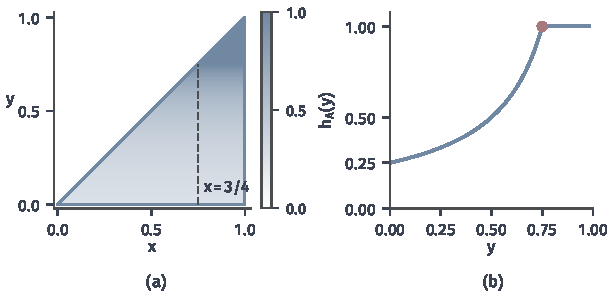
\includegraphics[width=104mm]{figures/07-probability/02-measure-theoretic-probability/matplotlib/cdis-event-function/figure.pdf}
  \caption{三角形模型中的条件概率$\mathbb{P}(X\in A\mid Y)$，$A=[\tfrac34,1]$。(a)三角形内一点$(x,y)$的颜色深浅表示$h_A(y)$，由白到蓝逐渐增大；颜色只随$y$变化，虚线$x=\tfrac34$左侧的点不在事件$\{X\in A\}$中，却与右侧同一水平线上的点取相同的值。(b)蓝线是$h_A(y)$，红点标出$y=\tfrac34$，此后$h_A=1$。}
  \label{fig:cdis-event-function}
\end{BookInlineFigure}

\paragraph{逐事件的概率规则}
条件概率是否像概率一样运算？非负、总量为一可以从条件期望的保序与线性直接得到；可数可加涉及无穷和，需要一个与积分的单调收敛定理对应的结论。

\begin{lemma}[条件单调收敛]
\label{lem:cdis-conditional-monotone}
设$0\leq Z_1\leq Z_2\leq\cdots$，$Z_n\to Z$，且$\mathbb{E}[Z]<\infty$。则$\mathbb{E}[Z_n\mid\mathcal{G}]$几乎必然递增地收敛到$\mathbb{E}[Z\mid\mathcal{G}]$。
\end{lemma}

\begin{proof}
由条件期望的保序性，对每个$n$，几乎必然有
\[
 0\leq\mathbb{E}[Z_n\mid\mathcal{G}]\leq\mathbb{E}[Z_{n+1}\mid\mathcal{G}]\leq\mathbb{E}[Z\mid\mathcal{G}].
\]
这是可数多个关系，例外集的并$N$仍是零概率集，并且$N\in\mathcal{G}$，因为它由$\mathcal{G}$可测的函数之间的比较定义。

在$N$之外令$W=\lim_n\mathbb{E}[Z_n\mid\mathcal{G}]$，在$N$上令$W=0$。$W$是$\mathcal{G}$可测函数的极限，因而$\mathcal{G}$可测，并且$0\leq W\leq\mathbb{E}[Z\mid\mathcal{G}]$几乎必然，所以可积。任取$G\in\mathcal{G}$，对递增的非负列两次使用单调收敛定理，得到
\[
 \mathbb{E}[\mathbf{1}_{G}W]=\lim_{n\to\infty}\mathbb{E}\bigl[\mathbf{1}_{G}\,\mathbb{E}[Z_n\mid\mathcal{G}]\bigr]=\lim_{n\to\infty}\mathbb{E}[\mathbf{1}_{G}Z_n]=\mathbb{E}[\mathbf{1}_{G}Z].
\]
中间的等号是条件期望在$G$上的积分恒等式。$W$满足条件期望的定义，由唯一性，$W=\mathbb{E}[Z\mid\mathcal{G}]$几乎必然。
\end{proof}

\begin{lemma}[逐事件的条件概率规则]
\label{lem:cdis-eventwise-rules}
对任意$A\in\mathcal{F}_{\mathcal{X}}$，几乎必然有$0\leq\mathbb{P}(X\in A\mid\mathcal{G})\leq1$，且$\mathbb{P}(X\in\mathcal{X}\mid\mathcal{G})=1$。对任意一列两两不交的$A_1,A_2,\ldots\in\mathcal{F}_{\mathcal{X}}$，几乎必然有
\begin{equation}
 \mathbb{P}\Bigl(X\in\bigcup_{n}A_n\Bigm|\mathcal{G}\Bigr)=\sum_{n}\mathbb{P}(X\in A_n\mid\mathcal{G}).
 \label{eq:cdis-eventwise-additivity}
\end{equation}
\end{lemma}

\begin{proof}
$0\leq\mathbf{1}_{\{X\in A\}}\leq1$，由保序性得到第一条；$\mathbf{1}_{\{X\in\mathcal{X}\}}=1$是常数，常数的条件期望是它自己。对不交的$A_n$，部分和$\sum_{k\leq n}\mathbf{1}_{\{X\in A_k\}}$递增地收敛到$\mathbf{1}_{\{X\in\cup_kA_k\}}$。由线性，部分和的条件期望是各项条件期望之和；再由引理~\ref{lem:cdis-conditional-monotone}取极限，得到式~\eqref{eq:cdis-eventwise-additivity}。
\end{proof}

引理中的“几乎必然”有一个容易忽略的限定：例外集依赖于所取的事件或事件列。对每个固定的$A$，总可以在一个零概率集之外谈论$\mathbb{P}(X\in A\mid Y=y)$；可是事件有不可数多个，不同事件的例外集合并起来可能不再是零概率集。于是出现一个问题：能否为每个$A$选定一个版本$h_A$，使对每个（或几乎每个）观测值$y$，映射$A\mapsto h_A(y)$都是$\mathcal{X}$上的一个概率分布？下面先给这样的对象一个名称。

\subsection{概率核}
\label{sec:cdis-kernel}

概率表给出了最简单的模型。传感器表按列$y$取出、除以列和，得到三个条件分布；把它们排成矩阵，每一行对应一个观测值，每行非负且和为$1$。这样的矩阵同时记录了所有目标事件的条件概率：给定$Y=y$时$X\in A$的概率，就是第$y$行在$A$中的元素之和。

\begin{BookInlineFigure}
  \centering
  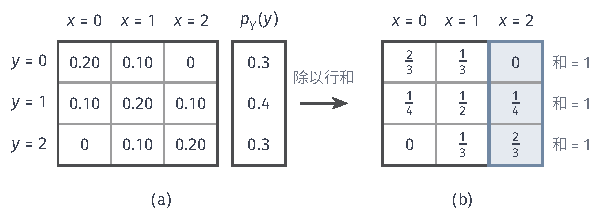
\includegraphics[width=102mm]{figures/07-probability/02-measure-theoretic-probability/tikz/cdis-table-kernel/figure.pdf}
  \caption{由传感器的联合概率表得到概率核。(a)联合概率表，行是第二台读数$y$，列是第一台读数$x$，右侧是行和$p_Y(y)$。(b)每行除以行和得到的矩阵$K(y,\{x\})$，每行是一个概率分布；浅蓝格子组成事件$\{X=2\}$所在的列，它的各行元素就是$\mathbb{P}(X=2\mid Y=y)$。}
  \label{fig:cdis-table-kernel}
\end{BookInlineFigure}

图~\ref{fig:cdis-table-kernel}画出这一步。对$A=\{2\}$，(b)中浅蓝一列给出$0,\tfrac14,\tfrac23$，正是上一小节逐个算出的条件概率；对其他事件，只要换成对应的列求和。一般情形要求的就是这样一个按观测值排列的分布族。

\begin{definition}[概率核]
\label{def:cdis-kernel}
设映射$K$对每个$y\in\mathcal{Y}$与$A\in\mathcal{F}_{\mathcal{X}}$给出一个数$K(y,A)\in[0,1]$。若
\begin{enumerate}
 \item 对每个$y\in\mathcal{Y}$，$A\mapsto K(y,A)$是$(\mathcal{X},\mathcal{F}_{\mathcal{X}})$上的概率测度；
 \item 对每个$A\in\mathcal{F}_{\mathcal{X}}$，$y\mapsto K(y,A)$是$\mathcal{F}_{\mathcal{Y}}$可测函数，
\end{enumerate}
则称$K$为从$(\mathcal{Y},\mathcal{F}_{\mathcal{Y}})$到$(\mathcal{X},\mathcal{F}_{\mathcal{X}})$的\term{概率核}（probability kernel），也称转移核。按测度的写法，$K(y,A)$也写成
\begin{equation}
 K(y,A)=\int_{A}K(y,\mathrm{d}x).
 \label{eq:cdis-kernel-notation}
\end{equation}
\end{definition}

两项要求各有用处。第一项是概率表“每行归一”的推广：固定观测值，得到一个完整的分布，事件之间的可加性对这个$y$处处成立，不再附带依赖事件的例外集。第二项保证固定事件$A$后，$K(\cdot,A)$是$\mathcal{Y}$上的可测函数，因而可以按$Y$的分布积分，例如计算$\int_{B}K(y,A)\,P_Y(\mathrm{d}y)$。$\mathcal{Y}$有限且每个子集都可测时，第二项自动成立，所以在概率表中只看得到第一项。

第二项并非多余。设$S\subseteq[0,1]$不是Borel集，令$y\in S$时$K(y,\cdot)$是$\{1\}$上的单点分布，其余$y$时是$\{0\}$上的单点分布。每个$K(y,\cdot)$都是概率测度，但$y\mapsto K(y,\{1\})=\mathbf{1}_{S}(y)$不可测，积分$\int K(y,\{1\})\,P_Y(\mathrm{d}y)$没有意义。这样的$K$无法用来“按观测加权”，也就谈不上与联合规律相容。

\paragraph{三角形模型的核}
三角形模型中，对$0\leq y<1$令$K(y,\cdot)$为$[y,1]$上的均匀分布，记$\lambda$为长度，则
\[
 K(y,A)=\frac{\lambda(A\cap[y,1])}{1-y},\qquad 0\leq y<1,
\]
在$y=1$等其余点令$K(y,\cdot)$为$\{1\}$上的单点分布。固定$y$，这是一个概率测度。固定$A$，函数$y\mapsto\lambda(A\cap[y,1])$连续，因而$K(\cdot,A)$在$[0,1)$上可测，补上可测的余下部分后整体可测。

图~\ref{fig:cdis-kernel-views}从两个方向看同一个核。(a)固定观测值，曲线是分布函数$t\mapsto K(y,[0,t])$：每个$y$对应一个完整的分布。(b)固定事件，曲线是观测值的函数$y\mapsto K(y,A)$：每个事件对应一个可测函数。概率核的定义就是要求这两个方向同时成立。

\begin{BookInlineFigure}
  \centering
  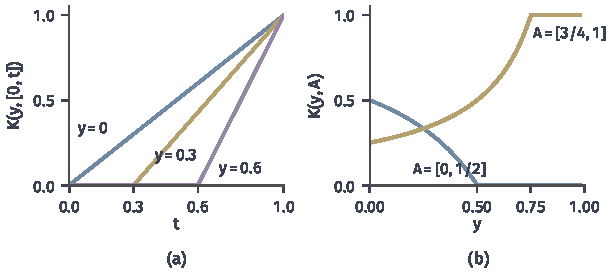
\includegraphics[width=104mm]{figures/07-probability/02-measure-theoretic-probability/matplotlib/cdis-kernel-views/figure.pdf}
  \caption{三角形模型的概率核$K(y,\cdot)=\operatorname{Unif}(y,1)$的两种读法。(a)固定$y=0,0.3,0.6$（蓝、黄、紫），横轴为$t$，曲线为$K(y,[0,t])$，每条都是一个分布函数。(b)固定事件$A=[0,\tfrac12]$（蓝）与$A=[\tfrac34,1]$（黄），曲线为$y\mapsto K(y,A)$。}
  \label{fig:cdis-kernel-views}
\end{BookInlineFigure}

\paragraph{核对函数与对测度的作用}
概率表的核是行和为一的非负矩阵，它可以从右边乘列向量，也可以从左边乘行向量。一般的核同样有这两种作用。对有界可测函数$g$，令$(Kg)(y)=\int g(x)\,K(y,\mathrm{d}x)$，这是“观测为$y$时$g$的平均”；对$\mathcal{Y}$上的概率测度$\mu$，令$(\mu K)(A)=\int K(y,A)\,\mu(\mathrm{d}y)$，这是“先按$\mu$抽观测值、再按核抽目标”时目标的分布。第~\ref{sec:cdis-integration}节与第~\ref{sec:cdis-joint}节分别研究这两种作用；概率表中它们就是矩阵乘列向量与行向量乘矩阵。

\subsection{正则条件分布}
\label{sec:cdis-regular}

概率核本身只是一族按观测值排列的分布，与$X$、$Y$的联合规律还没有关系。任意一个核都满足定义~\ref{def:cdis-kernel}，例如对所有$y$都取同一个分布。要让它成为“给定$Y$时$X$的分布”，必须要求它在每个事件上给出的值就是条件概率。

\begin{definition}[正则条件分布]
\label{def:cdis-regular}
从$\mathcal{Y}$到$\mathcal{X}$的概率核$K$若对每个$A\in\mathcal{F}_{\mathcal{X}}$满足
\begin{equation}
 K(Y,A)=\mathbb{P}(X\in A\mid Y)\quad\text{几乎必然},
 \label{eq:cdis-regular}
\end{equation}
则称$K$为给定$Y$时$X$的\term{正则条件分布}（regular conditional distribution），也记作$P_{X\mid Y}(A\mid y)=K(y,A)$。
\end{definition}

式~\eqref{eq:cdis-regular}中的例外集仍然可以随$A$改变，这一点与逐事件的条件概率相同。差别在于，核对每个$y$都是概率测度：正则条件分布是从条件概率的众多版本中挑出的一组，使得在每个观测值处都拼成一个分布。“正则”指的就是这种可以拼合的性质。给定一般的信息$\mathcal{G}$时，把$\mathcal{Y}$换成$(\Omega,\mathcal{G})$、$Y$换成恒等映射，同样可以定义给定$\mathcal{G}$的正则条件分布，本章主要讨论给定随机对象$Y$的情形。

验证一个核是否满足式~\eqref{eq:cdis-regular}，按条件期望的定义需要检查$\sigma(Y)$中的每个事件。$\sigma(Y)$的事件都形如$\{Y\in B\}$，把这一检查写成$\mathcal{Y}$上的积分，得到一个便于计算的判别。

\begin{lemma}[正则条件分布的积分判别]
\label{lem:cdis-regular-criterion}
概率核$K$是给定$Y$时$X$的正则条件分布，当且仅当对一切$A\in\mathcal{F}_{\mathcal{X}}$、$B\in\mathcal{F}_{\mathcal{Y}}$，
\begin{equation}
 \mathbb{P}(X\in A,\ Y\in B)=\int_{B}K(y,A)\,P_Y(\mathrm{d}y).
 \label{eq:cdis-regular-criterion}
\end{equation}
\end{lemma}

\begin{proof}
固定$A$。$K(\cdot,A)$可测且取值于$[0,1]$，所以$K(Y,A)$是$\sigma(Y)$可测的有界随机变量。按条件期望的定义，式~\eqref{eq:cdis-regular}成立当且仅当对每个$\{Y\in B\}\in\sigma(Y)$，
\[
 \mathbb{E}\bigl[\mathbf{1}_{\{Y\in B\}}K(Y,A)\bigr]=\mathbb{E}\bigl[\mathbf{1}_{\{Y\in B\}}\mathbf{1}_{\{X\in A\}}\bigr].
\]
右边是$\mathbb{P}(X\in A,\ Y\in B)$。左边的被积函数是$Y$的函数$\mathbf{1}_{B}(y)K(y,A)$，由分布的积分公式（第~\ref{chap:probability-spaces}章），它等于$\int_{B}K(y,A)\,P_Y(\mathrm{d}y)$。两边相等就是式~\eqref{eq:cdis-regular-criterion}。
\end{proof}

式~\eqref{eq:cdis-regular-criterion}说的是：按观测的分布把各个$y$处的条件概率加权累计，必须回到联合概率。这正是“条件化是缩小样本范围再重新归一”的反向检验：把各组重新归一的结果乘回组的质量，应当恢复原来的质量分配。

\paragraph{与概率表和条件密度相容}
有概率表时，取$K(y,\{x\})=p_{X,Y}(x,y)/p_Y(y)$（$p_Y(y)>0$），$p_Y(y)=0$的$y$上任取一个分布。代入式~\eqref{eq:cdis-regular-criterion}的右边，零概率的$y$不贡献，于是
\[
 \sum_{y\in B}p_Y(y)\sum_{x\in A}\frac{p_{X,Y}(x,y)}{p_Y(y)}=\sum_{y\in B}\sum_{x\in A}p_{X,Y}(x,y)=\mathbb{P}(X\in A,\ Y\in B).
\]
第~\ref{chap:random-vectors}章的条件质量函数确实给出正则条件分布。

三角形模型中，$P_Y$有密度$f_Y(y)=2(1-y)$。代入上一小节的核，对$y<1$，$K(y,A)f_Y(y)=2\lambda(A\cap[y,1])$，所以
\[
 \int_{B}K(y,A)\,f_Y(y)\,\mathrm{d}y=\int_{B}\int_{A}2\cdot\mathbf{1}_{\{x\geq y\}}\,\mathrm{d}x\,\mathrm{d}y=\mathbb{P}(X\in A,\ Y\in B).
\]
最后一步是联合密度在$A\times B$上的积分，交换次序的依据是Tonelli定理。一般的条件密度公式在第~\ref{sec:cdis-zero-probability}小节用同样的方法验证。

\paragraph{没有联合密度的情形}
密度比并不是正则条件分布的必要形式。设$Y\sim\operatorname{Unif}(0,1)$，$X=Y$。$(X,Y)$的全部质量落在对角线上，对角线的面积为零，联合密度不存在。直觉上，知道$Y=y$就知道$X=y$，所以应取$K(y,\cdot)=\delta_y$，即$\{y\}$上的单点分布。核对式~\eqref{eq:cdis-regular-criterion}：
\[
 \int_{B}\delta_y(A)\,P_Y(\mathrm{d}y)=P_Y(A\cap B)=\mathbb{P}(Y\in A,\ Y\in B)=\mathbb{P}(X\in A,\ Y\in B).
\]
式~\eqref{eq:cdis-regular-criterion}成立。核$\delta_y$可测：$y\mapsto\delta_y(A)=\mathbf{1}_{A}(y)$对Borel集$A$是可测函数。这个例子说明，正则条件分布的定义不依赖密度，只依赖联合规律本身。


\section{存在性与版本}
\label{sec:cdis-existence}

正则条件分布要求一个概率核同时给出所有事件的条件概率。逐事件的条件概率总是存在，但每个都只在各自的零概率集之外唯一，拼合时可能出问题。这一节先用一个例子说明随意挑选版本会怎样失败，再给出正则条件分布存在的条件，然后说明它在什么意义下唯一，最后讨论单个零概率观测值上的取值。

\subsection{存在条件}
\label{sec:cdis-existence-conditions}

\paragraph{随意挑选版本的失败}
仍取$Y\sim\operatorname{Unif}(0,1)$、$X=Y$。对每个单点$a\in[0,1]$，事件$\{X=a\}$的概率为零，指示函数几乎必然为零，所以常数$0$是$\mathbb{P}(X=a\mid Y)$的一个合法版本，即可以取$h_{\{a\}}\equiv0$。对每个区间$I$，取$h_{I}(y)=\mathbf{1}_{I}(y)$，这也是合法版本。

现在固定任意一个观测值$y$，看这些版本能否在$y$处拼成一个分布。若概率测度$\mu$在所有区间上满足$\mu(I)=\mathbf{1}_{I}(y)$，则$\mu$与$\delta_y$在区间上相同；区间对有限交封闭并生成Borel集，由测度在生成$\pi$系统上的唯一性，$\mu=\delta_y$，于是$\mu(\{y\})=1$。可是挑出的版本给单点$\{y\}$的值是$0$。这组版本在\emph{每一个}$y$处都拼不成分布，见图~\ref{fig:cdis-version-collapse}。

\begin{BookInlineFigure}
  \centering
  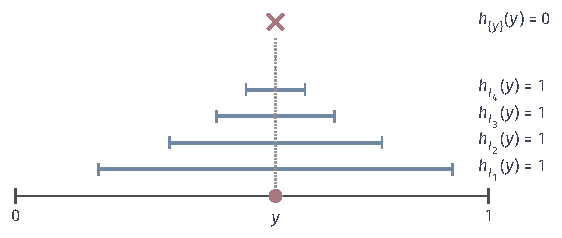
\includegraphics[width=95mm]{figures/07-probability/02-measure-theoretic-probability/tikz/cdis-version-collapse/figure.pdf}
  \caption{随意挑选版本的失败，$X=Y\sim\operatorname{Unif}(0,1)$。固定观测值$y$（红点），包含$y$的区间（蓝线）逐个缩小，所选版本都给出$1$；单点$\{y\}$所选的版本是$0$（红叉）。可数可加性要求区间上的值递减到单点上的值，二者矛盾。}
  \label{fig:cdis-version-collapse}
\end{BookInlineFigure}

每个单点事件的版本只在零概率集$\{Y=a\}$上“出错”，单独看都没有问题；不可数多个这样的零概率集合并起来却覆盖了整个$[0,1]$。补救的思路是：只对可数个事件选版本，可数个零概率集的并仍是零概率集；再用这可数个事件把整个分布确定下来。在实轴上，有理数处的分布函数值就足够确定一个分布。

\paragraph{实值目标}
先处理$X$取实数值的情形。观测$Y$的取值空间不需要任何结构。

\begin{theorem}[实值随机变量的正则条件分布]
\label{thm:cdis-existence-real}
设$X$是实随机变量，$Y$取值于任意可测空间$(\mathcal{Y},\mathcal{F}_{\mathcal{Y}})$。则存在给定$Y$时$X$的正则条件分布，即存在从$\mathcal{Y}$到$(\mathbb{R},\mathcal{B}(\mathbb{R}))$的概率核$K$，使对每个Borel集$A$，$K(Y,A)=\mathbb{P}(X\in A\mid Y)$几乎必然成立。
\end{theorem}

\begin{proof}
证明分四步：在有理数上选版本，收集可数个关系，修正成分布函数，最后核对可测性与版本性质。

第一步，选版本。对每个有理数$q$，由式~\eqref{eq:cdis-function-representation}取可测函数$G_q:\mathcal{Y}\to[0,1]$，使$G_q(Y)=\mathbb{P}(X\leq q\mid Y)$几乎必然。

第二步，收集关系。下面每条都由一个已知结论保证几乎必然成立：
\begin{enumerate}
 \item 对有理数$q<r$，$G_q(Y)\leq G_r(Y)$，由条件期望的保序性；
 \item 对每个有理数$q$，$G_{q+1/n}(Y)\to G_q(Y)$（$n\to\infty$），对递增到$\mathbf{1}_{\{X>q\}}$的$\mathbf{1}_{\{X>q+1/n\}}$用引理~\ref{lem:cdis-conditional-monotone}，再用线性；
 \item $G_{-n}(Y)\to0$，$G_{n}(Y)\to1$（$n\to\infty$），理由同上。
\end{enumerate}
令$N$为使上述某条关系不成立的$y$的全体。每条关系不成立的$y$构成$\mathcal{F}_{\mathcal{Y}}$中的可测集，因为它们由可数个可测函数$G_q$定义；关系几乎必然成立，说明这个集合的$P_Y$测度为零。关系一共可数条，所以$N$可测，并且$P_Y(N)=0$。

第三步，修正。对$y\notin N$，令
\[
 F(t\mid y)=\inf\{G_q(y):q\in\mathbb{Q},\ q>t\},\qquad t\in\mathbb{R}.
\]
由第1条，$F(\cdot\mid y)$不减；作为$q>t$上的下确界，它右连续。由第1、2条，在有理数$q$处$F(q\mid y)=\lim_nG_{q+1/n}(y)=G_q(y)$。由第3条，$t\to-\infty$时$F\to0$，$t\to+\infty$时$F\to1$。所以$F(\cdot\mid y)$是一个分布函数，对应$\mathbb{R}$上唯一的概率测度，记为$K(y,\cdot)$。对$y\in N$，令$K(y,\cdot)=\delta_0$。

第四步，核对。先看可测性。对实数$t$，取有理数$q_n\downarrow t$，则
\[
 K(y,(-\infty,t])=\mathbf{1}_{N^{\mathrm{c}}}(y)\lim_{n\to\infty}G_{q_n}(y)+\mathbf{1}_{N}(y)\,\mathbf{1}_{\{t\geq0\}},
\]
是可测函数的极限与组合，所以可测。使$y\mapsto K(y,A)$可测的Borel集$A$的全体对补集（$K(y,A^{\mathrm{c}})=1-K(y,A)$）和不交可数并（可测函数之和）封闭，含$\mathbb{R}$，是$\lambda$系统；它包含对有限交封闭的半直线族，由$\pi$--$\lambda$定理包含全部Borel集。

再看版本性质。对有理数$q$，在$\{Y\notin N\}$上$K(Y,(-\infty,q])=G_q(Y)$，所以$K(Y,(-\infty,q])=\mathbb{P}(X\leq q\mid Y)$几乎必然。对实数$t$与$q_n\downarrow t$，左边由测度的连续性收敛到$K(Y,(-\infty,t])$，右边由第二步的同一论证几乎必然收敛到$\mathbb{P}(X\leq t\mid Y)$，两者几乎必然相等。使$K(Y,A)=\mathbb{P}(X\in A\mid Y)$几乎必然成立的$A$的全体，由线性与引理~\ref{lem:cdis-eventwise-rules}对补集和不交可数并封闭，同样是含半直线族的$\lambda$系统，于是包含全部Borel集。
\end{proof}

证明的关键在第二步：所有要求都写成可数条，例外集只并了可数次。第三步的下确界把“只在有理数上知道的值”补成右连续的分布函数，在例外集$N$上则直接换成一个固定的分布。图~\ref{fig:cdis-rational-thresholds}用三角形模型画出这两种情形。

\begin{BookInlineFigure}
  \centering
  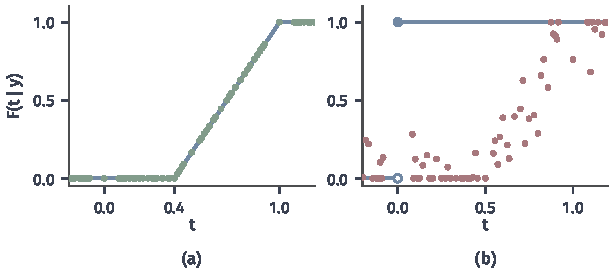
\includegraphics[width=104mm]{figures/07-probability/02-measure-theoretic-probability/matplotlib/cdis-rational-thresholds/figure.pdf}
  \caption{由有理阈值构造条件分布函数（三角形模型）。(a)$y=0.4$不在例外集中：绿点是分母不超过$12$的有理数$q$处的值$G_q(y)$，蓝线是由下确界得到的$F(t\mid y)$，即$[0.4,1]$上均匀分布的分布函数。(b)在一个零概率的观测值上，若所选版本的值（红点）不单调，该点划入例外集，改用固定的分布$\delta_0$（蓝线）。}
  \label{fig:cdis-rational-thresholds}
\end{BookInlineFigure}

\paragraph{标准Borel空间}
证明只用到实轴的两个性质：有一列可数的事件生成全部Borel集，并且在这列事件上相容的值能补成一个测度。许多取值空间可以搬到实轴上而保留这些性质。

\begin{definition}[标准Borel空间]
\label{def:cdis-standard-borel}
可测空间$(\mathcal{X},\mathcal{F}_{\mathcal{X}})$若存在Borel集$S\subseteq\mathbb{R}$与双射$\varphi:\mathcal{X}\to S$，使$\varphi$与$\varphi^{-1}$都可测（$S$取相对Borel $\sigma$代数），则称它为\term{标准Borel空间}（standard Borel space），$\varphi$称为\term{Borel同构}（Borel isomorphism）。
\end{definition}

有限集与可数集（每个子集都可测）满足定义：把元素依次编号为$1,2,\dots$，编号映射与它的逆都可测。更一般地，带Borel $\sigma$代数的完备可分度量空间都是标准Borel空间，其中包括$\mathbb{R}^{d}$、矩阵空间、它们的Borel子集，以及标准Borel空间的可数乘积。这一结论的证明需要用到描述集合论中关于Borel集像的定理，篇幅较长，读者可查阅~\scite{math-kallenberg2021probability}。

它的含义可以从$[0,1)^{2}$看出。把两个坐标写成二进制小数，再把两串数字交替排成一串，就得到$[0,1)$中的一个数，见图~\ref{fig:cdis-digit-interleave}。这个映射把平面上的点一对一地编成一个实数，前$2k$位数字只依赖两个坐标的前$k$位，所以它和它的逆都可测。证明中需要额外处理的只是二进制展开不唯一的那些点，它们构成一个可数集。

\begin{BookInlineFigure}
  \centering
  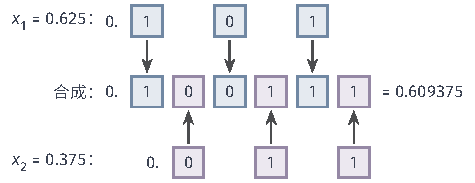
\includegraphics[width=80mm]{figures/07-probability/02-measure-theoretic-probability/tikz/cdis-digit-interleave/figure.pdf}
  \caption{交替排列二进制数字，把$[0,1)^{2}$中的点$(x_1,x_2)$编成$[0,1)$中的一个数。蓝色数字是$x_1=0.625$的二进制位，紫色数字是$x_2=0.375$的二进制位，两串数字$101$与$011$交替排成$100111$，合成的二进制小数$0.100111$等于$0.609375$。}
  \label{fig:cdis-digit-interleave}
\end{BookInlineFigure}

\begin{theorem}[正则条件分布的存在性]
\label{thm:cdis-existence}
设$X$取值于标准Borel空间$(\mathcal{X},\mathcal{F}_{\mathcal{X}})$，$Y$取值于任意可测空间$(\mathcal{Y},\mathcal{F}_{\mathcal{Y}})$，特别地，$\mathcal{Y}$可以是标准Borel空间。则给定$Y$时$X$的正则条件分布存在。
\end{theorem}

\begin{proof}
取Borel同构$\varphi:\mathcal{X}\to S$，令$X'=\varphi(X)$，它是实随机变量。由定理~\ref{thm:cdis-existence-real}，存在给定$Y$时$X'$的正则条件分布$K'$。因为$X'\in S$必然成立，$K'(Y,S)=\mathbb{P}(X'\in S\mid Y)=1$几乎必然，于是集合$N=\{y:K'(y,S)<1\}$可测且$P_Y(N)=0$。

固定一点$x_0\in\mathcal{X}$，令
\[
 K(y,A)=\begin{cases}K'\bigl(y,\varphi(A)\bigr), & y\notin N,\\ \delta_{x_0}(A), & y\in N.\end{cases}
\]
$\varphi(A)=(\varphi^{-1})^{-1}(A)$是$S$的Borel子集，所以右边有意义。$y\notin N$时，$K'(y,\cdot)$的质量全在$S$上，$\varphi$又是双射，$A\mapsto K'(y,\varphi(A))$就是$K'(y,\cdot)$在$S$上的部分经$\varphi^{-1}$推前得到的概率测度。可测性由$K'$继承。最后，$\{X\in A\}=\{X'\in\varphi(A)\}$，所以
\[
 \begin{aligned}
 K(Y,A)&=K'\bigl(Y,\varphi(A)\bigr)=\mathbb{P}\bigl(X'\in\varphi(A)\bigm|Y\bigr)\\
 &=\mathbb{P}(X\in A\mid Y)\quad\text{几乎必然}.
 \end{aligned}\qedhere
\]
\end{proof}

比较一下两种存在性。对单个可积随机变量，条件期望总是存在，第~\ref{chap:conditional-expectation}章用Radon--Nikodym定理构造它，不要求取值空间有任何结构。正则条件分布要把不可数多个条件概率拼在一起，需要目标空间提供一列可数的生成事件以及从这些事件上的值恢复测度的能力；标准Borel条件同时提供了这两点。在没有这类结构的一般可测空间上，可以构造出正则条件分布不存在的例子，构造要用到不可测集，篇幅较长。本卷遇到的取值空间（实数、向量、矩阵、有限或可数的符号集，以及它们的有限或可数乘积）都是标准Borel空间，以后把这一条件作为默认设定，在需要时说明。

\subsection{几乎处处唯一性}
\label{sec:cdis-uniqueness}

正则条件分布找到了一个，是否还有别的？在一个$P_Y$零测集上改动核，积分判别~\eqref{eq:cdis-regular-criterion}察觉不到，问题是除此之外还有没有更大的自由。

\begin{theorem}[正则条件分布的几乎处处唯一性]
\label{thm:cdis-uniqueness}
设$X$取值于标准Borel空间，$K$与$K'$都是给定$Y$时$X$的正则条件分布。则存在$N\in\mathcal{F}_{\mathcal{Y}}$，$P_Y(N)=0$，使对一切$y\notin N$，$K(y,\cdot)=K'(y,\cdot)$。
\end{theorem}

\begin{proof}
先取一个可数且对有限交封闭的事件族$\mathcal{P}$，它生成$\mathcal{F}_{\mathcal{X}}$。$\mathcal{X}=\mathbb{R}$时取$\{(-\infty,q]:q\in\mathbb{Q}\}$；一般情形取Borel同构$\varphi$，令$\mathcal{P}$为这些半直线的原像$\varphi^{-1}((-\infty,q])$的全体，$q\in\mathbb{Q}$。

对每个$P\in\mathcal{P}$，两个核都是$\mathbb{P}(X\in P\mid Y)$的版本，所以$K(Y,P)=K'(Y,P)$几乎必然，即集合$N_P=\{y:K(y,P)\neq K'(y,P)\}$满足$P_Y(N_P)=0$。令$N=\bigcup_{P\in\mathcal{P}}N_P$，它是可数个零测集的并，$P_Y(N)=0$。对$y\notin N$，两个概率测度$K(y,\cdot)$与$K'(y,\cdot)$在生成$\pi$系统$\mathcal{P}$上取值相同，由测度在生成$\pi$系统上的唯一性（可参考\BookChapterRef{chap:measure}{卷四第5章“测度”}），它们在$\mathcal{F}_{\mathcal{X}}$上相同。
\end{proof}

与存在性的证明一样，关键是把比较压缩到可数个事件上，使例外集只并可数次。结论中的例外集用观测的分布$P_Y$来衡量，而不是用$\mathcal{Y}$上的某种“体积”。

\paragraph{单个观测值上的取值}
定理~\ref{thm:cdis-uniqueness}的反面同样重要：联合规律只决定核的$P_Y$等价类，不决定它在某个特定零测点上的值。三角形模型中，把$y=\tfrac12$处的分布换成$\delta_0$，得到核$K'$。$P_Y(\{\tfrac12\})=0$，式~\eqref{eq:cdis-regular-criterion}中积分不受影响，$K'$仍是正则条件分布；可是$K'(\tfrac12,\cdot)$说“给定$Y=\tfrac12$时$X=0$”，而$X\geq Y$本应必然成立。同样可以在所有有理数$y$上改动，甚至在零测的Cantor集上改动。

改动不能扩大到正测度的观测集上。若在$y\in[\tfrac14,\tfrac12]$上把核换成$\operatorname{Unif}(0,1)$，取$A=[0,\tfrac18]$、$B=[\tfrac14,\tfrac12]$。三角形中$X\geq Y\geq\tfrac14$，所以$\mathbb{P}(X\in A,\ Y\in B)=0$，而改动后的核给出
\[
 \int_{1/4}^{1/2}\frac18\cdot2(1-y)\,\mathrm{d}y=\frac14\int_{1/4}^{1/2}(1-y)\,\mathrm{d}y=\frac14\cdot\frac{5}{32}=\frac{5}{128}>0 ,
\]
式~\eqref{eq:cdis-regular-criterion}不成立。图~\ref{fig:cdis-two-versions}对照了两种改动。

\begin{BookInlineFigure}
  \centering
  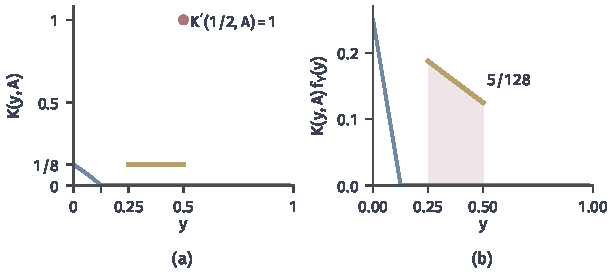
\includegraphics[width=104mm]{figures/07-probability/02-measure-theoretic-probability/matplotlib/cdis-two-versions/figure.pdf}
  \caption{三角形模型中$A=[0,\tfrac18]$时核的几种取法。(a)蓝线是由密度比得到的$y\mapsto K(y,A)$，在$y\geq\tfrac18$时为零；红点是只在$y=\tfrac12$一个点上的改动，它仍给出正则条件分布；黄线把$[\tfrac14,\tfrac12]$整段改成$\tfrac18$。(b)式~\eqref{eq:cdis-regular-criterion}中的被积函数$K(y,A)f_Y(y)$：单点改动不影响积分，黄线的改动多出浅红区域的质量$\tfrac{5}{128}$，不再是正则条件分布。}
  \label{fig:cdis-two-versions}
\end{BookInlineFigure}

若某个观测值本身有正概率，$P_Y(\{y_0\})>0$，它不可能落在零测例外集中，$K(y_0,\cdot)$就被唯一确定，并且由式~\eqref{eq:cdis-regular-criterion}取$B=\{y_0\}$，
\[
 K(y_0,A)=\frac{\mathbb{P}(X\in A,\ Y=y_0)}{\mathbb{P}(Y=y_0)},
\]
这正是第~\ref{chap:classical-probability}章的条件概率。正则条件分布在有正概率的观测值上与初等条件概率一致，额外的自由只出现在零概率的观测值上。

\subsection{零概率条件}
\label{sec:cdis-zero-probability}

$Y$连续时，每个单点的概率都是零，$\mathbb{P}(X\in A\mid Y=y)$不能写成两个事件概率之比。正则条件分布给这个记号一个意义：它就是$K(y,A)$，作为$y$的函数在$P_Y$几乎处处的意义下由联合规律确定。下面先说明密度公式给出一个版本，再讨论单个零概率观测值上附加的选择。

\paragraph{密度公式给出的版本}
设$\alpha,\beta$分别是$\mathcal{X},\mathcal{Y}$上的$\sigma$有限测度，例如Lebesgue测度或计数测度，$(X,Y)$关于乘积测度$\alpha\otimes\beta$有联合密度$f$。记$f_Y(y)=\int f(x,y)\,\alpha(\mathrm{d}x)$为$Y$关于$\beta$的密度。

\begin{theorem}[条件密度给出的正则条件分布]
\label{thm:cdis-density-version}
在上述设定下，任取$\mathcal{X}$上的概率测度$\nu_0$，令
\begin{equation}
 K(y,A)=\begin{cases}
 \dfrac{1}{f_Y(y)}\displaystyle\int_{A}f(x,y)\,\alpha(\mathrm{d}x), & 0<f_Y(y)<\infty,\\
 \nu_0(A), & \text{其他}.
 \end{cases}
 \label{eq:cdis-density-version}
\end{equation}
则$K$是给定$Y$时$X$的正则条件分布。
\end{theorem}

\begin{proof}
对$0<f_Y(y)<\infty$的$y$，$K(y,\cdot)$是非负函数$f(\cdot,y)/f_Y(y)$关于$\alpha$的不定积分，总量为$1$，是概率测度；其余$y$处是$\nu_0$。由Tonelli定理，$y\mapsto\int_{A}f(x,y)\,\alpha(\mathrm{d}x)$与$f_Y$都可测，集合$\{0<f_Y<\infty\}$可测，所以$K(\cdot,A)$可测，$K$是概率核。

再核对式~\eqref{eq:cdis-regular-criterion}。$\int f_Y\,\mathrm{d}\beta=1$，所以$\{f_Y=\infty\}$是$\beta$零测集；$\{f_Y=0\}$上被积函数含因子$f_Y=0$。于是这两部分都不贡献，
\[
 \begin{aligned}
 \int_{B}K(y,A)\,f_Y(y)\,\beta(\mathrm{d}y)&=\int_{B}\int_{A}f(x,y)\,\alpha(\mathrm{d}x)\,\beta(\mathrm{d}y)\\
 &=\mathbb{P}(X\in A,\ Y\in B).
 \end{aligned}
\]
由引理~\ref{lem:cdis-regular-criterion}，$K$是正则条件分布。
\end{proof}

定理同时涵盖了概率表（$\alpha,\beta$都取计数测度）、条件密度（都取Lebesgue测度），以及离散状态与连续读数的混合模型（一个取计数测度，一个取Lebesgue测度）。证明没有用到标准Borel条件：有了联合密度，核可以直接写出来。

公式~\eqref{eq:cdis-density-version}在每个$y$处都给出一个值，但这个值依赖所选的密度$f$。联合密度只在$\alpha\otimes\beta$零测集之外确定；在直线$\{y=y_0\}$上任意改动$f$，联合规律不变，$K(y_0,\cdot)$却变了。单个零概率观测值上的条件分布需要额外的要求来选定。

\paragraph{连续性的要求}
常用的要求是连续性。第~\ref{chap:random-vectors}章证明：若联合密度在$y_0$附近连续且$f_Y(y_0)>0$，窄带$\{y_0\leq Y\leq y_0+h\}$上的条件概率在$h\to0$时趋于密度比。这个极限选出了一个特定的值。设$\mathcal{Y}=\mathbb{R}$。若两个版本对定理~\ref{thm:cdis-uniqueness}证明中可数生成族的每个事件$P$，$y\mapsto K(y,P)$都在$y_0$处连续，并且$y_0$的每个邻域都有正的$P_Y$质量，那么两个版本在$y_0$处相同：它们在一个$P_Y$零测集之外相等，每个邻域里都有这样的点，取极限即得两者在每个$P$上的值相同，再由生成$\pi$系统上的唯一性得到$K(y_0,\cdot)$相同。

这种选择有两个限度。其一，满足要求的版本未必存在。设$Y\sim\operatorname{Unif}(-1,1)$，$X=\mathbf{1}_{\{Y>0\}}$。正则条件分布在$y<0$时是$\delta_0$，在$y>0$时是$\delta_1$（几乎处处唯一），$y=0$处无论取什么，$y\mapsto K(y,\{1\})$都不连续，见图~\ref{fig:cdis-no-continuous}。连续性在这里无法选出$K(0,\cdot)$，这一点的值只能另作约定。

\begin{BookInlineFigure}
  \centering
  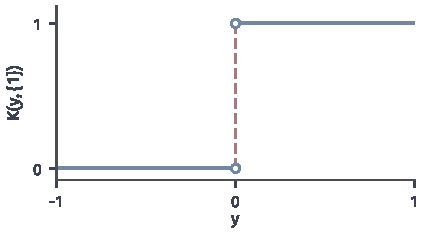
\includegraphics[width=72mm]{figures/07-probability/02-measure-theoretic-probability/matplotlib/cdis-no-continuous/figure.pdf}
  \caption{$Y\sim\operatorname{Unif}(-1,1)$、$X=\mathbf{1}_{\{Y>0\}}$时的$y\mapsto K(y,\{1\})$。蓝线在$y<0$时为$0$，在$y>0$时为$1$；$y=0$处（红色虚线上的任何值）怎样取都不能使它连续。}
  \label{fig:cdis-no-continuous}
\end{BookInlineFigure}

其二，选出的值依赖用哪个观测量逼近同一个零概率事件。设$(X,Y)$在单位正方形上均匀分布，问“给定$X=Y$时$X$的分布”。事件$\{X=Y\}$可以写成$\{D=0\}$，其中$D=Y-X$；也可以写成$\{R=1\}$，其中$R=Y/X$。两种写法描述同一条对角线，给出的条件分布却不同。

\paragraph{两种逼近的计算}
先用$D$。由换元$(x,y)\mapsto(x,d)=(x,y-x)$，Jacobian行列式为$1$，$(X,D)$的联合密度是
\[
 f_{X,D}(x,d)=1,\qquad 0<x<1,\ 0<x+d<1 .
\]
在$d=0$处它对$x\in(0,1)$恒为$1$，边缘$f_D(0)=1$，由式~\eqref{eq:cdis-density-version}，给定$D=0$时$X$的条件密度是$1$，即$X\sim\operatorname{Unif}(0,1)$。

再用$R$。由换元$(x,y)\mapsto(x,r)=(x,y/x)$，逆变换$y=rx$的Jacobian行列式为$x$，$(X,R)$的联合密度是
\[
 f_{X,R}(x,r)=x,\qquad 0<x<1,\ 0<rx<1 .
\]
在$r=1$处它是$x$，边缘$f_R(1)=\int_0^1x\,\mathrm{d}x=\tfrac12$，所以给定$R=1$时$X$的条件密度是$2x$。两个结果都由连续的联合密度得到，都是各自观测量下“连续性选出的”版本，却互不相同。

图~\ref{fig:cdis-borel-kolmogorov}说明差别从哪里来。$\{\lvert D\rvert\leq h\}$是沿对角线等宽的带子，各处收进同样多的质量；$\{\lvert R-1\rvert\leq h\}$是从原点张开的楔形，离原点越远越宽，收进的质量与$x$成正比。两种窄化在极限下落在同一条线上，但沿线分配质量的权重不同。这一现象称为\term{Borel--Kolmogorov悖论}（Borel--Kolmogorov paradox）。

\begin{BookInlineFigure}
  \centering
  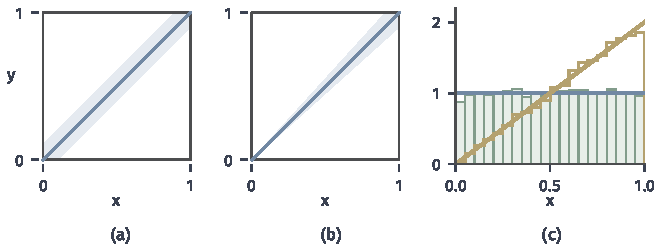
\includegraphics[width=112mm]{figures/07-probability/02-measure-theoretic-probability/matplotlib/cdis-borel-kolmogorov/figure.pdf}
  \caption{同一条对角线的两种逼近，$(X,Y)$在单位正方形上均匀分布。(a)浅蓝带子$\{\lvert Y-X\rvert\leq h\}$，$h=0.1$。(b)浅蓝楔形$\{\lvert Y/X-1\rvert\leq h\}$，$h=0.1$。(c)固定种子$7$模拟$4\times10^{5}$个点，取$h=0.02$：落在带子中的点的$X$坐标直方图为浅绿柱，落在楔形中的为黄色阶梯线；蓝线与黄线是极限密度$1$与$2x$。}
  \label{fig:cdis-borel-kolmogorov}
\end{BookInlineFigure}

悖论并不说明理论有矛盾。条件分布总是“给定某个观测量$Y$”的分布，它是$\mathcal{Y}$上的一个核，只在$P_Y$几乎处处的意义下确定。$D$与$R$是两个不同的观测量，生成不同的信息，给定$D$与给定$R$的条件分布是两个不同的核；它们在各自零概率点$d=0$、$r=1$上的值，分别依赖各自的选择方式。脱离观测量单独说“给定零概率事件$\{X=Y\}$”，没有确定的意义。在零概率观测值上用连续性等要求选值时，必须指明观测量，核对满足要求的版本存在，并清楚所得的值是一种约定，而不是由联合规律推出的结论。


\section{条件分布的积分}
\label{sec:cdis-integration}

固定观测值$y$，$K(y,\cdot)$是一个普通的概率测度，可以对它积分。这样得到的$\int g(x)\,K(y,\mathrm{d}x)$是“观测为$y$时$g(X)$的平均”。它与第~\ref{chap:conditional-expectation}章的条件期望$\mathbb{E}[g(X)\mid Y]$是什么关系？这一节证明，在可积条件下两者几乎必然相等，再用这个表示计算条件矩。

条件期望仍以第~\ref{chap:conditional-expectation}章的积分刻画为定义，它对任何可积随机变量都存在；下面的表示只在正则条件分布存在时才可用，它提供的是一个计算方法和一个对每个$y$都有定义的版本。

\subsection{条件期望的积分表示}
\label{sec:cdis-integral-representation}

\begin{theorem}[条件期望的积分表示]
\label{thm:cdis-integral-representation}
设$K$是给定$Y$时$X$的正则条件分布，$g:\mathcal{X}\to\mathbb{R}$可测，$\mathbb{E}\lvert g(X)\rvert<\infty$。则对$P_Y$几乎每个$y$，$\int\lvert g(x)\rvert\,K(y,\mathrm{d}x)<\infty$，并且
\begin{equation}
 \mathbb{E}[g(X)\mid Y]=\int g(x)\,K(Y,\mathrm{d}x)\quad\text{几乎必然}.
 \label{eq:cdis-integral-representation}
\end{equation}
在使积分不收敛的$P_Y$零测集上，右边可以取任意常数，例如$0$。
\end{theorem}

证明沿着积分本身的构造进行：先对指示函数，再对简单函数，然后用单调极限处理非负函数，最后拆成正负两部分。两边的每一步分别用测度积分的性质与条件期望的性质。

\begin{proof}
记$(Kg)(y)=\int g(x)\,K(y,\mathrm{d}x)$。

第一步，$g=\mathbf{1}_{A}$。此时$(Kg)(Y)=K(Y,A)$，式~\eqref{eq:cdis-integral-representation}就是正则条件分布的定义~\eqref{eq:cdis-regular}。

第二步，$g=\sum_{i=1}^{m}c_i\mathbf{1}_{A_i}$是简单函数。左边由条件期望的线性，右边由积分的线性，都拆成各项之和，各项由第一步相等。

第三步，$g\geq0$。取简单函数$g_n=\min\{n,\ 2^{-n}\lfloor2^{n}g\rfloor\}$，它们非负、递增地收敛到$g$。对每个固定的$y$，由单调收敛定理（对测度$K(y,\cdot)$），
\[
 (Kg_n)(y)\uparrow(Kg)(y)\in[0,\infty],
\]
所以$Kg$作为可测函数的极限是可测的。另一方面$g(X)$可积，由引理~\ref{lem:cdis-conditional-monotone}，$\mathbb{E}[g_n(X)\mid Y]\uparrow\mathbb{E}[g(X)\mid Y]$几乎必然。由第二步两列的每一项几乎必然相等，极限也几乎必然相等，这就是式~\eqref{eq:cdis-integral-representation}。

再看有限性。对$(Kg_n)(Y)$取期望，用全期望公式与第二步，$\mathbb{E}[(Kg_n)(Y)]=\mathbb{E}[g_n(X)]$；两边对$n$用单调收敛定理，得到
\[
 \int(Kg)(y)\,P_Y(\mathrm{d}y)=\mathbb{E}[g(X)]<\infty .
\]
非负函数的积分有限，它就只能在一个$P_Y$零测集上取$+\infty$。

第四步，一般的可积$g$。写$g=g^{+}-g^{-}$，两部分都非负且$g^{\pm}(X)$可积。由第三步，$Kg^{+}$与$Kg^{-}$在一个共同的$P_Y$零测集之外都有限，在这个零测集之外，$\lvert g\rvert$关于$K(y,\cdot)$的积分是$(Kg^{+})(y)+(Kg^{-})(y)<\infty$，并且$(Kg)(y)=(Kg^{+})(y)-(Kg^{-})(y)$。再由条件期望的线性，
\[
 \mathbb{E}[g(X)\mid Y]=\mathbb{E}[g^{+}(X)\mid Y]-\mathbb{E}[g^{-}(X)\mid Y]=(Kg)(Y)\quad\text{几乎必然}. \qedhere
\]
\end{proof}

第三步的单调逼近可以具体地看。三角形模型中取$y=0.4$，$K(0.4,\cdot)$是$[0.4,1]$上的均匀分布，取$g(x)=x^{2}$。精确值是
\[
 \int x^{2}\,K(0.4,\mathrm{d}x)=\frac{1}{0.6}\int_{0.4}^{1}x^{2}\,\mathrm{d}x=\frac{1-0.064}{1.8}=0.52 .
\]
$g$不超过$1$，所以$g_n=2^{-n}\lfloor2^{n}g\rfloor$，它是$2^{n}$级的阶梯。$n=1,2,3,4$时，阶梯函数在$K(0.4,\cdot)$下的积分依次约为
\[
 0.244,\qquad 0.386,\qquad 0.456,\qquad 0.488,
\]
递增地逼近$0.52$，见图~\ref{fig:cdis-simple-approx}。

\begin{BookInlineFigure}
  \centering
  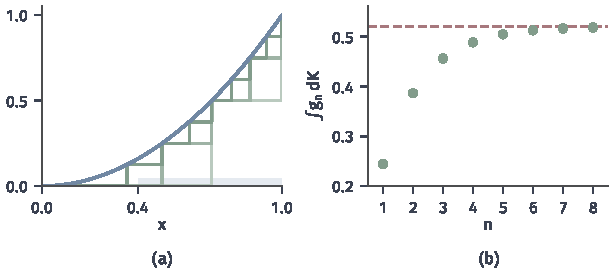
\includegraphics[width=104mm]{figures/07-probability/02-measure-theoretic-probability/matplotlib/cdis-simple-approx/figure.pdf}
  \caption{用简单函数逼近条件分布下的积分，三角形模型，$y=0.4$。(a)蓝线是$g(x)=x^{2}$，绿色阶梯是$g_n=2^{-n}\lfloor2^{n}g\rfloor$（$n=1,2,3$，颜色由浅到深），浅蓝区间$[0.4,1]$是$K(0.4,\cdot)$的支撑。(b)绿点是$\int g_n\,\mathrm{d}K(0.4,\cdot)$，$n=1,\dots,8$，红色虚线是极限$0.52$。}
  \label{fig:cdis-simple-approx}
\end{BookInlineFigure}

\paragraph{离散与密度的情形}
把定理~\ref{thm:cdis-integral-representation}用于前面的两类模型，就得到熟悉的公式。有概率表时，对$p_Y(y)>0$，
\[
 \mathbb{E}[g(X)\mid Y=y]=\sum_{x}g(x)\,\frac{p_{X,Y}(x,y)}{p_Y(y)} ;
\]
有联合密度时，由定理~\ref{thm:cdis-density-version}，对$0<f_Y(y)<\infty$，
\[
 \mathbb{E}[g(X)\mid Y=y]=\int g(x)\,\frac{f_{X,Y}(x,y)}{f_Y(y)}\,\mathrm{d}x .
\]
第~\ref{chap:random-vectors}章按这两个公式计算条件均值，当时它们只是“组内平均”的计算规则；现在可以说，它们给出的函数代入$Y$后正是条件期望的一个版本，第~\ref{chap:conditional-expectation}章关于条件期望的全部性质都可以用于它们。

三角形模型中，对$0\leq y<1$，
\[
 \mathbb{E}[g(X)\mid Y=y]=\frac{1}{1-y}\int_{y}^{1}g(x)\,\mathrm{d}x ,
\]
即$[y,1]$上$g$的平均值。取$g(x)=x$得到$(1+y)/2$，与第~\ref{chap:random-vectors}章的结果一致。

\subsection{条件矩的计算}
\label{sec:cdis-conditional-moments}

设$X$是实随机变量。取$g(x)=x^{k}$或$g(x)=\lvert x\rvert^{p}$，在相应的矩存在时，定理~\ref{thm:cdis-integral-representation}给出条件矩的积分公式：若$\mathbb{E}\lvert X\rvert^{p}<\infty$，$p>0$，则
\begin{equation}
 \mathbb{E}\bigl[\lvert X\rvert^{p}\bigm|Y\bigr]=\int\lvert x\rvert^{p}\,K(Y,\mathrm{d}x)<\infty\quad\text{几乎必然},
 \label{eq:cdis-conditional-abs-moment}
\end{equation}
若$k\leq p$是正整数，则几乎必然
\[
 \mathbb{E}[X^{k}\mid Y]=\int x^{k}\,K(Y,\mathrm{d}x),
\]
其中$\lvert x\rvert^{k}\leq1+\lvert x\rvert^{p}$保证$X^{k}$可积。这些量称为给定$Y$的\term{条件矩}（conditional moment）。

\paragraph{条件方差}
第~\ref{chap:conditional-expectation}章对$\mathbb{E}[X^{2}]<\infty$定义了条件方差
\[
 \operatorname{Var}(X\mid Y)=\mathbb{E}\bigl[(X-\mathbb{E}[X\mid Y])^{2}\bigm|Y\bigr].
\]
记$m(y)=\int x\,K(y,\mathrm{d}x)$，它在$P_Y$几乎每个$y$处有限，并且$m(Y)=\mathbb{E}[X\mid Y]$几乎必然。条件方差可以写成条件分布的方差。

\begin{theorem}[条件方差的积分表示]
\label{thm:cdis-conditional-variance}
设$\mathbb{E}[X^{2}]<\infty$，$K$是给定$Y$时$X$的正则条件分布。则几乎必然
\begin{equation}
 \operatorname{Var}(X\mid Y)=\int\bigl(x-m(Y)\bigr)^{2}\,K(Y,\mathrm{d}x)=\int x^{2}\,K(Y,\mathrm{d}x)-m(Y)^{2}.
 \label{eq:cdis-conditional-variance}
\end{equation}
\end{theorem}

\begin{proof}
由式~\eqref{eq:cdis-conditional-abs-moment}，存在$P_Y$零测集$N$，使$y\notin N$时$\int x^{2}\,K(y,\mathrm{d}x)<\infty$，从而$m(y)$有限。对这样的$y$，$K(y,\cdot)$是二阶矩有限的分布，展开平方得到
\[
 \begin{aligned}
 \int\bigl(x-m(y)\bigr)^{2}K(y,\mathrm{d}x)&=\int x^{2}K(y,\mathrm{d}x)-2m(y)^{2}+m(y)^{2}\\
 &=\int x^{2}K(y,\mathrm{d}x)-m(y)^{2}.
 \end{aligned}
\]
这是式~\eqref{eq:cdis-conditional-variance}的第二个等号。

另一方面，展开条件方差的定义。$m(Y)$与$X$都平方可积，由Cauchy--Schwarz不等式$m(Y)X$可积，于是可以用线性和提取已知量：
\[
 \begin{aligned}
 \operatorname{Var}(X\mid Y)&=\mathbb{E}[X^{2}\mid Y]-2m(Y)\,\mathbb{E}[X\mid Y]+m(Y)^{2}\\
 &=\mathbb{E}[X^{2}\mid Y]-m(Y)^{2}.
 \end{aligned}
\]
由式~\eqref{eq:cdis-conditional-abs-moment}取$p=2$，右边第一项$\mathbb{E}[X^{2}\mid Y]$几乎必然等于$\int x^{2}K(Y,\mathrm{d}x)$，两式相同。
\end{proof}

式~\eqref{eq:cdis-conditional-variance}就是“方差等于二阶矩减均值平方”对每个条件分布分别使用。它把条件方差从一个由积分刻画定义的随机变量，变成了每个观测值处一个具体分布的方差。

\paragraph{正面概率随机的硬币}
设$U\sim\operatorname{Unif}(0,1)$，给定$U=u$时把一枚正面概率为$u$的硬币独立地抛$n$次，$N$是正面次数。这句话本身就是用概率核描述的模型：
\[
 K(u,\{k\})=\binom{n}{k}u^{k}(1-u)^{n-k},\qquad k=0,1,\dots,n ,
\]
即给定$U=u$时$N\sim\operatorname{Bin}(n,u)$。联合规律由$U$的分布和这个核共同确定，第~\ref{sec:cdis-joint}节说明为什么这样确定的联合规律唯一，并且这个核就是它的正则条件分布。

二项分布的均值与方差在第~\ref{chap:common-distributions}章已经算出，代入式~\eqref{eq:cdis-integral-representation}与式~\eqref{eq:cdis-conditional-variance}，
\[
 \mathbb{E}[N\mid U]=nU,\qquad \operatorname{Var}(N\mid U)=nU(1-U).
\]
条件均值随$U$线性增长，条件方差在$U=\tfrac12$处最大，在两端趋于零。

由全方差公式，总方差是条件方差的平均加上条件均值的方差。用$\mathbb{E}[U]=\tfrac12$、$\mathbb{E}[U^{2}]=\tfrac13$、$\operatorname{Var}(U)=\tfrac1{12}$，
\[
 \mathbb{E}\bigl[nU(1-U)\bigr]=n\Bigl(\frac12-\frac13\Bigr)=\frac n6,\qquad \operatorname{Var}(nU)=\frac{n^{2}}{12}.
\]
于是
\[
 \operatorname{Var}(N)=\frac n6+\frac{n^{2}}{12}=\frac{n(n+2)}{12}.
\]
$n=10$时组内部分为$\tfrac53\approx1.67$，组间部分为$\tfrac{25}{3}\approx8.33$，总方差为$10$。组间部分随$n^{2}$增长，占了大头：抛得越多，正面次数的波动主要来自硬币本身的不确定，而不是给定硬币后的随机性。图~\ref{fig:cdis-coin-moments}画出这两部分。第~\ref{sec:cdis-mixture}小节将看到$N$在$\{0,1,\dots,n\}$上均匀分布，其方差$\bigl((n+1)^{2}-1\bigr)/12$与这里的结果相同。

\begin{BookInlineFigure}
  \centering
  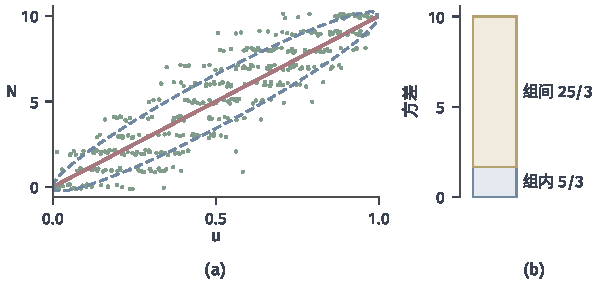
\includegraphics[width=104mm]{figures/07-probability/02-measure-theoretic-probability/matplotlib/cdis-coin-moments/figure.pdf}
  \caption{正面概率随机的硬币，$n=10$。(a)绿点是固定种子$3$模拟的$400$对$(U,N)$，纵向略加抖动以便看清；红线是条件均值$10u$，蓝色虚线是条件均值加减一个条件标准差$\sqrt{10u(1-u)}$。(b)总方差$10$的分解：浅蓝为组内部分$\tfrac53$，浅黄为组间部分$\tfrac{25}{3}$。}
  \label{fig:cdis-coin-moments}
\end{BookInlineFigure}

\paragraph{有限性只在几乎处处的意义下成立}
式~\eqref{eq:cdis-conditional-abs-moment}说整体矩有限保证条件矩\emph{几乎处处}有限，不能加强为对每个观测值有限。三角形模型中，把$y=\tfrac12$处的分布换成标准Cauchy分布，由第~\ref{sec:cdis-uniqueness}小节，所得的核仍是正则条件分布；可是Cauchy分布的绝对一阶矩是无穷，$\lvert x\rvert$关于$K'(\tfrac12,\cdot)$的积分发散，尽管$X$有界。哪个零测点上的条件矩有限，联合规律管不着。

反方向同样不成立：每个观测值上的条件矩有限，不能推出整体矩有限。设$Y\sim\operatorname{Unif}(0,1)$，给定$Y=y$时$X\sim\operatorname{Exp}(y)$，即率参数为$y$的指数分布。对每个$y\in(0,1)$，条件均值有限，
\[
 \int x\,K(y,\mathrm{d}x)=\frac1y<\infty .
\]
可是定理~\ref{thm:cdis-integral-representation}证明第三步中关于有限性的论证只用到简单函数与单调收敛，对任何非负$g$都成立，结果允许取$+\infty$：$\int(Kg)\,\mathrm{d}P_Y=\mathbb{E}[g(X)]$。取$g(x)=x$，
\[
 \mathbb{E}[X]=\int_0^1\frac1y\,\mathrm{d}y=+\infty .
\]
条件均值$1/y$在$y\to0$附近增长得太快，加权平均发散，见图~\ref{fig:cdis-moment-directions}。此时$X$不可积，第~\ref{chap:conditional-expectation}章的条件期望没有定义，只能说核的积分$1/y$是一个逐点有限的函数。

\begin{BookInlineFigure}
  \centering
  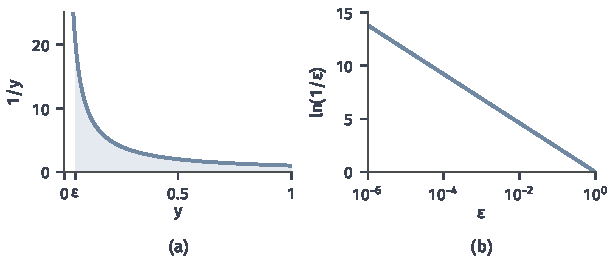
\includegraphics[width=104mm]{figures/07-probability/02-measure-theoretic-probability/matplotlib/cdis-moment-directions/figure.pdf}
  \caption{逐点有限的条件均值不保证整体可积。$Y\sim\operatorname{Unif}(0,1)$，给定$Y=y$时$X\sim\operatorname{Exp}(y)$。(a)蓝线是条件均值$1/y$，浅蓝区域是$[\varepsilon,1]$上的面积，$\varepsilon=0.05$。(b)蓝线是截断积分$\int_{\varepsilon}^{1}y^{-1}\,\mathrm{d}y=\ln(1/\varepsilon)$，横轴按对数刻度，$\varepsilon\to0$时无界增长。}
  \label{fig:cdis-moment-directions}
\end{BookInlineFigure}


\section{联合分布的分解}
\label{sec:cdis-joint}

上一节固定观测值，对条件分布积分。现在把观测值也放开，按观测的边缘分布再积分一次。概率表中，这相当于把条件分布的每一行乘回行的质量，恢复整张表；对列求和得到目标的边缘；逐个变量重复这一步，就能从头构造多个随机对象的联合规律。这一节依次落实这三件事，并说明每一步保留哪些条件变量。

\subsection{联合分布的恢复}
\label{sec:cdis-recovery}

引理~\ref{lem:cdis-regular-criterion}已经说明，矩形事件的联合概率可以由核与边缘恢复：
\[
 \mathbb{P}(X\in A,\ Y\in B)=\int_{B}K(y,A)\,P_Y(\mathrm{d}y).
\]
三角形模型中取$A=[\tfrac34,1]$、$B=[0,\tfrac12]$。对$y\leq\tfrac12$，$K(y,A)=\tfrac{1}{4(1-y)}$，乘以$f_Y(y)=2(1-y)$得到常数$\tfrac12$，所以
\[
 \mathbb{P}\bigl(X\geq\tfrac34,\ Y\leq\tfrac12\bigr)=\int_0^{1/2}\frac12\,\mathrm{d}y=\frac14 .
\]
直接计算，事件对应边长为$\tfrac14$与$\tfrac12$的矩形，它整个落在三角形内，面积$\tfrac18$乘以密度$2$也是$\tfrac14$，见图~\ref{fig:cdis-joint-recovery}。

\begin{BookInlineFigure}
  \centering
  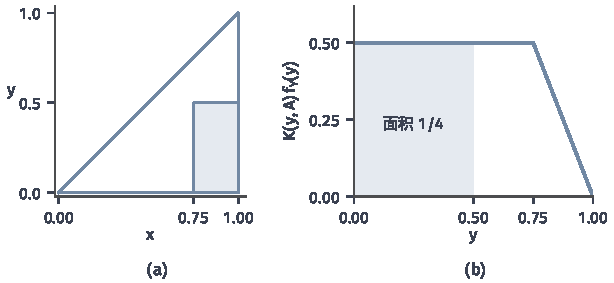
\includegraphics[width=104mm]{figures/07-probability/02-measure-theoretic-probability/matplotlib/cdis-joint-recovery/figure.pdf}
  \caption{由核与边缘恢复矩形事件的联合概率，三角形模型。(a)浅蓝矩形是事件$\{X\geq\tfrac34,\ Y\leq\tfrac12\}$，蓝线围成三角形。(b)蓝线是$y\mapsto K(y,A)f_Y(y)$，$A=[\tfrac34,1]$；它在$y\leq\tfrac34$时等于$\tfrac12$，此后等于$2(1-y)$。浅蓝区域是$[0,\tfrac12]$上的积分，面积为$\tfrac14$。}
  \label{fig:cdis-joint-recovery}
\end{BookInlineFigure}

矩形之外的事件，例如$\{X+Y\leq1\}$，以及一般的期望$\mathbb{E}[f(X,Y)]$，怎样由核与边缘算出？对乘积空间中的集合$E$，记它在$y$处的截面为$E^{y}=\{x:(x,y)\in E\}$。自然的猜测是先在每个$y$处按$K(y,\cdot)$量出截面，再按$Y$的分布累计。下面的定理说明这个猜测正确，并且由此定义的测度唯一。

\begin{theorem}[由核与边缘确定联合规律]
\label{thm:cdis-kernel-product}
设$\mu$是$\mathcal{Y}$上的概率测度，$K$是从$\mathcal{Y}$到$\mathcal{X}$的概率核。
\begin{enumerate}
 \item 对每个$E\in\mathcal{F}_{\mathcal{X}}\otimes\mathcal{F}_{\mathcal{Y}}$，$y\mapsto K(y,E^{y})$可测，并且
 \begin{equation}
  (\mu\otimes K)(E)=\int K(y,E^{y})\,\mu(\mathrm{d}y)
  \label{eq:cdis-kernel-product}
 \end{equation}
 是乘积空间上的概率测度。它是在每个可测矩形$A\times B$上取值$\int_{B}K(y,A)\,\mu(\mathrm{d}y)$的唯一概率测度。
 \item 对非负可测函数$f$，$y\mapsto\int f(x,y)\,K(y,\mathrm{d}x)$可测，并且
 \begin{equation}
  \int f\,\mathrm{d}(\mu\otimes K)=\int\!\!\int f(x,y)\,K(y,\mathrm{d}x)\,\mu(\mathrm{d}y).
  \label{eq:cdis-kernel-product-integral}
 \end{equation}
 若$f$关于$\mu\otimes K$可积，内层积分对$\mu$几乎每个$y$绝对收敛，式~\eqref{eq:cdis-kernel-product-integral}仍成立。
 \item 若$K$是给定$Y$时$X$的正则条件分布，则$P_Y\otimes K$就是$(X,Y)$的联合分布，从而对非负可测或使$f(X,Y)$可积的$f$，
 \begin{equation}
  \mathbb{E}[f(X,Y)]=\int\!\!\int f(x,y)\,K(y,\mathrm{d}x)\,P_Y(\mathrm{d}y).
  \label{eq:cdis-joint-recovery}
 \end{equation}
\end{enumerate}
\end{theorem}

\begin{proof}
第1条，先证可测性。令$\mathcal{D}$为使$y\mapsto K(y,E^{y})$可测的$E$的全体。对可测矩形，$(A\times B)^{y}$在$y\in B$时是$A$，否则是空集，所以$K(y,(A\times B)^{y})=K(y,A)\mathbf{1}_{B}(y)$可测，矩形属于$\mathcal{D}$。整个空间属于$\mathcal{D}$；补集的截面是截面的补集，$K(y,(E^{\mathrm{c}})^{y})=1-K(y,E^{y})$；两两不交的集合，截面也两两不交，$K(y,\cdot)$可数可加，所得的函数是可测函数之和。所以$\mathcal{D}$是$\lambda$系统。可测矩形对有限交封闭并生成乘积$\sigma$代数，由$\pi$--$\lambda$定理，$\mathcal{D}$包含全部可测集。

再证式~\eqref{eq:cdis-kernel-product}定义了概率测度。空集的截面都是空集，全空间的截面都是$\mathcal{X}$，所以测度分别为$0$和$1$。对两两不交的$E_n$，截面两两不交，
\[
 (\mu\otimes K)\Bigl(\bigcup_nE_n\Bigr)=\int\sum_{n}K(y,E_n^{y})\,\mu(\mathrm{d}y)=\sum_{n}(\mu\otimes K)(E_n),
\]
逐项积分的依据是单调收敛定理。取$E=A\times B$，式~\eqref{eq:cdis-kernel-product}给出$\int_{B}K(y,A)\,\mu(\mathrm{d}y)$。两个概率测度若在可测矩形上相同，由生成$\pi$系统上的唯一性，它们相同。

第2条，按积分的构造进行。$f=\mathbf{1}_{E}$时，内层积分是$K(y,E^{y})$，结论就是第1条。简单函数由线性得到。非负可测$f$取简单函数$f_n\uparrow f$：每个$y$处内层积分由单调收敛定理递增收敛，极限可测；外层再用一次单调收敛定理。$f$可积时，分别处理$f^{+}$与$f^{-}$；由非负情形，$\int\!\int\lvert f\rvert\,K(y,\mathrm{d}x)\,\mu(\mathrm{d}y)<\infty$，所以内层的$\int\lvert f(x,y)\rvert\,K(y,\mathrm{d}x)$只在$\mu$零测集上为无穷。

第3条，由引理~\ref{lem:cdis-regular-criterion}，$(X,Y)$的联合分布在每个可测矩形上的取值与$P_Y\otimes K$相同，由第1条的唯一性两者相同。式~\eqref{eq:cdis-joint-recovery}是第2条对联合分布的改写，其左边由分布的积分公式写成期望。
\end{proof}

定理与卷四的Tonelli、Fubini定理结构相同，可参考\BookChapterRef{chap:integration}{卷四第6章“积分”}。乘积测度是$K(y,\cdot)$不随$y$改变的特例：此时$\mu\otimes K$就是两个测度的乘积，$X$与$Y$独立。一般的核让截面的“量法”随$y$改变，这正是依赖关系的来源。

\paragraph{一个非矩形的例子}
用式~\eqref{eq:cdis-joint-recovery}计算三角形模型中的$\mathbb{E}[XY]$。内层对$x$积分时把$y$当作常数，由第~\ref{sec:cdis-integral-representation}小节，$\int x\,K(y,\mathrm{d}x)=(1+y)/2$，于是
\[
 \int x y\,K(y,\mathrm{d}x)=\frac{y(1+y)}{2}.
\]
再按$f_Y(y)=2(1-y)$积分，
\[
 \mathbb{E}[XY]=\int_0^1\frac{y(1+y)}{2}\cdot2(1-y)\,\mathrm{d}y=\int_0^1(y-y^{3})\,\mathrm{d}y=\frac14 .
\]
直接用联合密度计算，结果相同：
\[
 \int_0^1\int_0^{x}2xy\,\mathrm{d}y\,\mathrm{d}x=\int_0^1x^{3}\,\mathrm{d}x=\frac14 .
\]

\paragraph{给定观测时代入观测值}
定理~\ref{thm:cdis-kernel-product}还给出了一个常用的计算规则：求$f(X,Y)$给定$Y$的条件期望时，可以把$Y$的观测值代入，只对$X$按条件分布积分。设$\mathbb{E}\lvert f(X,Y)\rvert<\infty$，则
\begin{equation}
 \mathbb{E}[f(X,Y)\mid Y]=\int f(x,Y)\,K(Y,\mathrm{d}x)\quad\text{几乎必然}.
 \label{eq:cdis-substitution}
\end{equation}
右边由第2条是$Y$的可测函数。对$B\in\mathcal{F}_{\mathcal{Y}}$，把式~\eqref{eq:cdis-joint-recovery}用于$\mathbf{1}_{B}(y)f(x,y)$，得到右边在$\{Y\in B\}$上的积分等于$\mathbb{E}[\mathbf{1}_{\{Y\in B\}}f(X,Y)]$，这正是条件期望的积分刻画。例如$\mathbb{E}[XY\mid Y]=Y\,\mathbb{E}[X\mid Y]$，与提取已知量的规则一致。

\paragraph{不只是密度的乘法}
有联合密度时，式~\eqref{eq:cdis-joint-recovery}就是在$f_Y(y)>0$处把$f_{X,Y}$写成$f_Y(y)f_{X\mid Y}(x\mid y)$再作累次积分。定理本身不需要密度。图~\ref{fig:cdis-non-density}给出两个没有平面联合密度的例子。

\begin{BookInlineFigure}
  \centering
  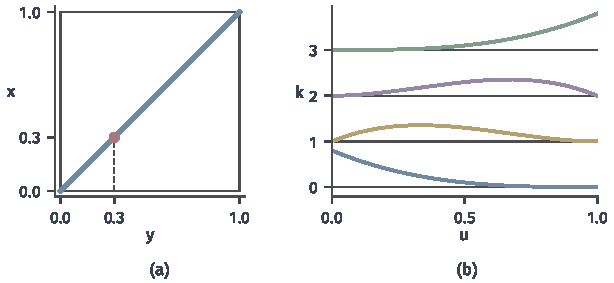
\includegraphics[width=104mm]{figures/07-probability/02-measure-theoretic-probability/matplotlib/cdis-non-density/figure.pdf}
  \caption{由核与边缘确定、但没有平面联合密度的联合规律。(a)$X=Y\sim\operatorname{Unif}(0,1)$：全部质量在蓝色对角线上，核$K(y,\cdot)=\delta_y$把$y=0.3$处的质量放在红点。(b)正面概率随机的硬币，$n=3$：$(U,N)$的质量分布在四条水平线$N=k$上，曲线是每条线上的密度$\binom{3}{k}u^{k}(1-u)^{3-k}$，$k=0,1,2,3$（蓝、黄、紫、绿）。}
  \label{fig:cdis-non-density}
\end{BookInlineFigure}

第一个例子是$X=Y\sim\operatorname{Unif}(0,1)$，核为$K(y,\cdot)=\delta_y$。由式~\eqref{eq:cdis-kernel-product}，$E^{y}$在$\delta_y$下的测度是$\mathbf{1}_{E}(y,y)$，所以
\[
 P_{(X,Y)}(E)=\int_0^1\mathbf{1}_{E}(y,y)\,\mathrm{d}y ,
\]
即质量沿对角线均匀分布。例如取$f(x,y)=(x-y)^{2}$，内层积分在每个$y$处都是$0$，所以$\mathbb{E}[(X-Y)^{2}]=0$。

第二个例子是硬币模型$(U,N)$，一个分量连续、一个分量离散。$N=k$的那条水平线上，质量关于$u$的密度是$\binom nk u^{k}(1-u)^{n-k}$；所有线上的密度对$u$积分再对$k$求和等于$1$。这两种联合规律都不是平面上的密度，却都由“边缘乘以核”唯一确定。

\subsection{全概率公式与混合分布}
\label{sec:cdis-mixture}

联合恢复公式中取$B=\mathcal{Y}$，即保留$X$的事件、对全部观测值积分，得到$X$的边缘分布：
\begin{equation}
 P_X(A)=\int K(y,A)\,P_Y(\mathrm{d}y),\qquad A\in\mathcal{F}_{\mathcal{X}} .
 \label{eq:cdis-total-probability}
\end{equation}
这是全概率公式的一般形式。第~\ref{chap:classical-probability}章的全概率公式把样本空间分成有限个正概率的组，再按组加权；这里的“组”是观测值$y$，可以有不可数多个，每组的概率可以为零，按$P_Y$加权的求和换成了积分。对函数，同样有$\mathbb{E}[g(X)]=\int(Kg)(y)\,P_Y(\mathrm{d}y)$，只要$g$非负或$g(X)$可积。

式~\eqref{eq:cdis-total-probability}也可以从另一个方向读：给定一族分布$\{K(y,\cdot)\}$和一个加权分布$\mu$，$\mu K$是一个新分布，称为这族分布按$\mu$的混合。$\mu$称为混合分布的权重，取值$y$称为混合变量。第~\ref{chap:random-vectors}章的房间温度模型就是两个分量的离散混合：$Y$表示房间状态，$\mu$给两种状态的概率$0.8$与$0.2$，$K$给出两个高斯分布，混合结果的密度是$0.8\,\phi(x-20)+0.2\,\phi(x-23)$。

\paragraph{连续混合：随机硬币的正面次数}
混合变量可以连续。硬币模型中，$U$的分布是$[0,1]$上的Lebesgue测度，代入式~\eqref{eq:cdis-total-probability}，
\[
 \mathbb{P}(N=k)=\int_0^1\binom nk u^{k}(1-u)^{n-k}\,\mathrm{d}u .
\]
由第~\ref{chap:common-distributions}章的Beta积分，对非负整数$a,b$，
\[
 \int_0^1u^{a}(1-u)^{b}\,\mathrm{d}u=\frac{a!\,b!}{(a+b+1)!},
\]
代入得到
\[
 \mathbb{P}(N=k)=\frac{n!}{k!\,(n-k)!}\cdot\frac{k!\,(n-k)!}{(n+1)!}=\frac{1}{n+1},\qquad k=0,1,\dots,n .
\]
正面次数在$\{0,1,\dots,n\}$上均匀分布。每个分量$\operatorname{Bin}(n,u)$都集中在$nu$附近，$u$均匀地扫过$[0,1]$，峰的位置也均匀地扫过$0$到$n$，叠加起来恰好铺平，见图~\ref{fig:cdis-mixtures}(a)。

\paragraph{连续混合：正态尺度混合}
第~\ref{chap:multivariate-distributions}章的多元t分布是另一个连续混合。那里$U\sim\chi^{2}_{\nu}$，给定$U=u$时$\bm{X}\sim\mathcal{N}\bigl(\bm{\mu},(\nu/u)\bm{\Sigma}\bigr)$，即核$K(u,\cdot)$是一族尺度不同的高斯分布。式~\eqref{eq:cdis-total-probability}给出
\[
 P_{\bm{X}}(S)=\int_0^{\infty}K(u,S)\,P_U(\mathrm{d}u),
\]
再对每个$K(u,\cdot)$的密度$g_u$用Tonelli定理交换积分，就得到那一章的混合密度：$\bm{X}$的密度是各分量密度$g_u(\bm{x})$按$P_U$的加权积分。这里的推导不需要$U$有密度：把尺度的分布换成任何$(0,\infty)$上的分布，例如只取两个值，混合仍有密度，只要每个分量有密度且$u\mapsto g_u(\bm{x})$可测。

\begin{BookInlineFigure}
  \centering
  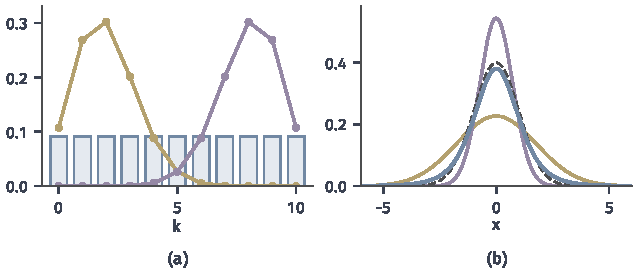
\includegraphics[width=108mm]{figures/07-probability/02-measure-theoretic-probability/matplotlib/cdis-mixtures/figure.pdf}
  \caption{两个连续混合。(a)$n=10$时的两个分量$\operatorname{Bin}(10,u)$，$u=0.2$（黄）与$u=0.8$（紫），以及对$u\in[0,1]$均匀混合后的分布，各点概率都是$1/11$（浅蓝柱）。(b)一元t分布作为正态尺度混合，$\nu=5$：黄、紫线是$U$取$\chi^{2}_{5}$的$10\%$与$90\%$分位数时的分量$\mathcal{N}(0,5/u)$，蓝线是混合得到的t密度，灰色虚线是$\mathcal{N}(0,1)$。}
  \label{fig:cdis-mixtures}
\end{BookInlineFigure}

图~\ref{fig:cdis-mixtures}(b)中，$u$较小的分量又宽又矮，$u$较大的分量窄而高；混合后的t密度中心比标准高斯略低，尾部明显更厚，厚尾来自那些尺度很大的分量。混合分布的矩也按条件矩加权：均值是条件均值的平均，方差由全方差公式分成组内与组间两部分，第~\ref{sec:cdis-conditional-moments}小节的硬币例子就是一次具体的计算。

\subsection{链式分解}
\label{sec:cdis-chain}

两个随机对象的联合规律可以分成“先$Y$、再给定$Y$的$X$”两步。有$n$个随机对象$X_1,\dots,X_n$时，可以依次进行：先定$X_1$，再给定$X_1$定$X_2$，再给定$(X_1,X_2)$定$X_3$，如此下去。每一步需要一个正则条件分布，它的存在由定理~\ref{thm:cdis-existence}保证，这里要求每个$X_k$取值于标准Borel空间$\mathcal{X}_k$。

记$\bm{x}_{1:k}=(x_1,\dots,x_k)$，$X_{1:k}=(X_1,\dots,X_k)$。下面的定理用到一个事实：标准Borel空间的有限乘积仍是标准Borel空间，这是第~\ref{sec:cdis-existence-conditions}小节所述可数乘积结论的特例。

\begin{theorem}[链式分解]
\label{thm:cdis-chain}
设$X_1,\dots,X_n$分别取值于标准Borel空间$\mathcal{X}_1,\dots,\mathcal{X}_n$。则存在概率核$K_k$（$k=2,\dots,n$），$K_k$从$\mathcal{X}_1\times\cdots\times\mathcal{X}_{k-1}$到$\mathcal{X}_k$，是给定$X_{1:k-1}$时$X_k$的正则条件分布；并且对非负可测函数$f$，
\begin{equation}
 \mathbb{E}[f(X_{1:n})]=\int P_{X_1}(\mathrm{d}x_1)\int K_2(x_1,\mathrm{d}x_2)\cdots\int K_n(\bm{x}_{1:n-1},\mathrm{d}x_n)\,f(\bm{x}_{1:n}).
 \label{eq:cdis-chain}
\end{equation}
反过来，任给$\mathcal{X}_1$上的概率测度$P_1$和这样的一列概率核$K_2,\dots,K_n$，式~\eqref{eq:cdis-chain}的右边（取$f$为指示函数）定义了乘积空间上唯一的概率测度；在这个测度下，坐标$X_1$的分布是$P_1$，$K_k$是给定$X_{1:k-1}$时$X_k$的正则条件分布。
\end{theorem}

\begin{proof}
对$n$归纳。$n=1$时式~\eqref{eq:cdis-chain}是分布的积分公式。设结论对$n-1$成立。$X_{1:n-1}$取值于标准Borel空间$\mathcal{X}_1\times\cdots\times\mathcal{X}_{n-1}$，由定理~\ref{thm:cdis-existence}，给定$X_{1:n-1}$时$X_n$的正则条件分布$K_n$存在。由定理~\ref{thm:cdis-kernel-product}第3条，取$Y=X_{1:n-1}$、$X=X_n$，
\[
 \mathbb{E}[f(X_{1:n})]=\int\Bigl(\int f(\bm{x}_{1:n-1},x_n)\,K_n(\bm{x}_{1:n-1},\mathrm{d}x_n)\Bigr)P_{X_{1:n-1}}(\mathrm{d}\bm{x}_{1:n-1}).
\]
括号内是$\bm{x}_{1:n-1}$的非负可测函数，对它用归纳假设展开外层积分，就得到式~\eqref{eq:cdis-chain}。

反方向同样归纳：由$P_1$与$K_2$，定理~\ref{thm:cdis-kernel-product}第1条给出$\mathcal{X}_1\times\mathcal{X}_2$上唯一的测度$\mu_2=P_1\otimes K_2$；再由$\mu_2$与$K_3$得到$\mu_3=\mu_2\otimes K_3$，依此类推。每一步的唯一性来自第1条。在$\mu_k$下，由第1条中的矩形公式与引理~\ref{lem:cdis-regular-criterion}，$K_k$是给定前$k-1$个坐标时第$k$个坐标的正则条件分布；后面各步只在前$k$个坐标之外添加新坐标，不改变前$k$个坐标的联合分布。
\end{proof}

正向的结论说，任何有限个标准Borel随机对象的联合规律都能逐次分解；反向的结论说，可以用起始分布和一列核逐步构造联合规律：先按$P_1$抽$x_1$，再按$K_2(x_1,\cdot)$抽$x_2$，再按$K_3(x_1,x_2,\cdot)$抽$x_3$。每一步的核都可以依赖已经得到的\emph{全部}取值。按这种方式实际产生样本的方法在第~\ref{chap:sample-generation}章研究。有联合密度时，式~\eqref{eq:cdis-chain}就是密度的连乘分解
\[
 f(\bm{x}_{1:n})=f_{X_1}(x_1)\,f_{X_2\mid X_1}(x_2\mid x_1)\cdots f_{X_n\mid X_{1:n-1}}(x_n\mid\bm{x}_{1:n-1}),
\]
在各边缘密度为正的范围内成立。

\paragraph{随机硬币的逐次抛掷}
回到正面概率为$U\sim\operatorname{Unif}(0,1)$的硬币，记第$k$次的结果为$X_k\in\{0,1\}$，$1$表示正面，给定$U=u$时各次独立且$\mathbb{P}(X_k=1\mid U=u)=u$。前$m$次中正面有$s$次的某个具体结果序列，概率是
\[
 \mathbb{P}(X_{1:m}=\bm{x}_{1:m})=\int_0^1u^{s}(1-u)^{m-s}\,\mathrm{d}u=\frac{s!\,(m-s)!}{(m+1)!}.
\]
它只依赖正面次数$s$，与正反面出现的次序无关。

给定前$k-1$次的结果，其中正面$s$次，第$k$次为正面的条件概率是两个这样的概率之比，取$m=k-1$：
\begin{equation}
 \mathbb{P}(X_k=1\mid X_{1:k-1}=\bm{x}_{1:k-1})=\frac{(s+1)!\,(k-1-s)!/(k+1)!}{s!\,(k-1-s)!/k!}=\frac{s+1}{k+1}.
 \label{eq:cdis-succession}
\end{equation}
这称为\term{Laplace继承法则}（Laplace's rule of succession）。先看到的正面越多，下一次越可能是正面：抛掷结果在不断透露$U$的信息。由于每个$\bm{x}_{1:k-1}$的概率为正，这里的核由初等条件概率唯一确定。

用链式分解计算$\mathbb{P}(X_1=1,X_2=1,X_3=0)$。三个因子依次由式~\eqref{eq:cdis-succession}取$k=1,2,3$得到：
\[
 \begin{gathered}
 \mathbb{P}(X_1=1)=\frac12,\qquad \mathbb{P}(X_2=1\mid X_1=1)=\frac23,\\
 \mathbb{P}(X_3=0\mid X_1=1,X_2=1)=1-\frac34=\frac14 .
 \end{gathered}
\]
相乘得到$\tfrac1{12}$，与直接积分的结果相同：
\[
 \int_0^1u^{2}(1-u)\,\mathrm{d}u=\frac13-\frac14=\frac1{12}.
\]
图~\ref{fig:cdis-succession-tree}画出全部八条路径。

\begin{BookInlineFigure}
  \centering
  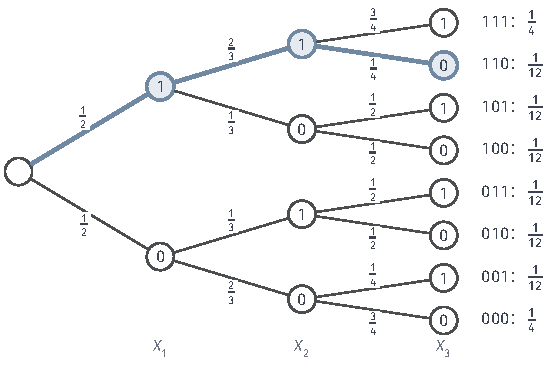
\includegraphics[width=94mm]{figures/07-probability/02-measure-theoretic-probability/tikz/cdis-succession-tree/figure.pdf}
  \caption{随机硬币前三次抛掷的链式分解。每条边上是由Laplace继承法则得到的条件概率，右侧是八个结果序列的概率；蓝色路径是$(1,1,0)$，概率为$\tfrac12\cdot\tfrac23\cdot\tfrac14=\tfrac1{12}$。}
  \label{fig:cdis-succession-tree}
\end{BookInlineFigure}

\paragraph{省去条件变量的后果}
式~\eqref{eq:cdis-chain}中每个核都给定了此前的全部变量。若为了简便，第三步只用$X_2$而忽略$X_1$，计算会出错。三次抛掷的联合规律在交换次序后不变，所以$(X_2,X_3)$与$(X_1,X_2)$同分布，
\[
 \mathbb{P}(X_3=0\mid X_2=1)=\mathbb{P}(X_2=0\mid X_1=1)=\frac13 ,
\]
于是“省略版”给出
\[
 \frac12\cdot\frac23\cdot\frac13=\frac19\neq\frac1{12}.
\]
差别的来源是：$X_1=1$与$X_2=1$合起来比单独的$X_2=1$透露了更多关于$U$的信息，使下一次出现反面的可能更小。图~\ref{fig:cdis-chain-omit}比较了八个序列在两种算法下的概率。省略版仍然给出一个总和为$1$的分布，所以无法从归一性看出错误。

\begin{BookInlineFigure}
  \centering
  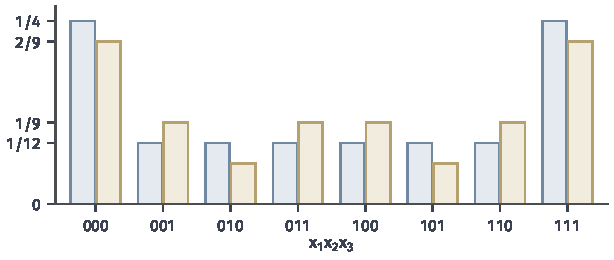
\includegraphics[width=104mm]{figures/07-probability/02-measure-theoretic-probability/matplotlib/cdis-chain-omit/figure.pdf}
  \caption{随机硬币三次抛掷的八个结果序列。蓝柱是由完整链式分解得到的真实概率，黄柱是第三步只给定$X_2$时的“省略版”概率；两组各自的和都是$1$，但在每个序列上都不相同。}
  \label{fig:cdis-chain-omit}
\end{BookInlineFigure}

一般地，把$K_k(\bm{x}_{1:k-1},\cdot)$换成只依赖其中一部分变量的核，是一个需要证明的断言：给定那部分变量以后，被省去的变量对$X_k$不再提供信息。这正是下一节的条件独立。


\section{条件独立}
\label{sec:cdis-conditional-independence}

上一节的硬币例子里，三次抛掷互不独立，可是一旦知道$U$，它们就是独立的抛掷：给定$U$以后，联合规律拆成了各次条件分布的乘积。什么时候给定一份信息以后，两个随机对象的联合规律可以这样拆开？拆开以后，链式分解中哪些条件变量可以省去？这一节先给出定义和判别，再看改变条件信息会怎样影响独立关系，最后用条件独立化简核的复合。

设$X,Z$分别取值于$(\mathcal{X},\mathcal{F}_{\mathcal{X}})$与$(\mathcal{Z},\mathcal{F}_{\mathcal{Z}})$，$\mathcal{G}$是子$\sigma$代数。

\subsection{定义与乘积分解}
\label{sec:cdis-ci-definition}

独立可以写成期望的乘积分解：对有界可测的$f,g$，
\[
 \mathbb{E}[f(X)g(Z)]=\mathbb{E}[f(X)]\,\mathbb{E}[g(Z)].
\]
把期望换成给定$\mathcal{G}$的条件期望，就得到给定信息后的版本。

\begin{definition}[条件独立]
\label{def:cdis-conditional-independence}
若对任意有界可测函数$f:\mathcal{X}\to\mathbb{R}$与$g:\mathcal{Z}\to\mathbb{R}$，
\begin{equation}
 \mathbb{E}[f(X)g(Z)\mid\mathcal{G}]=\mathbb{E}[f(X)\mid\mathcal{G}]\,\mathbb{E}[g(Z)\mid\mathcal{G}]\quad\text{几乎必然},
 \label{eq:cdis-conditional-independence}
\end{equation}
则称$X$与$Z$在给定$\mathcal{G}$时\term{条件独立}（conditionally independent），记作$X\perp\!\!\!\perp Z\mid\mathcal{G}$。$\mathcal{G}=\sigma(Y)$时记作$X\perp\!\!\!\perp Z\mid Y$。
\end{definition}

取$f=\mathbf{1}_{A}$、$g=\mathbf{1}_{C}$，定义包含了事件形式
\[
 \mathbb{P}(X\in A,\ Z\in C\mid\mathcal{G})=\mathbb{P}(X\in A\mid\mathcal{G})\,\mathbb{P}(Z\in C\mid\mathcal{G})\quad\text{几乎必然}.
\]
反过来，事件形式对一切$A,C$成立时，两边对$f,g$都是线性的，所以对简单函数成立；有界可测函数是简单函数的一致极限，而有界函数$h$的条件期望的绝对值几乎必然不超过$\sup\lvert h\rvert$，取极限即得式~\eqref{eq:cdis-conditional-independence}。$\mathcal{G}$只含零概率与全概率事件时，条件期望就是期望，条件独立回到独立。

\paragraph{条件联合分布的乘积}
给定观测$Y$、且$(X,Z)$有正则条件分布时，定义可以在每个观测值处读出来。设$\mathcal{X},\mathcal{Z}$都是标准Borel空间，$K$是给定$Y$时$(X,Z)$的正则条件分布。令
\[
 K_X(y,A)=K(y,A\times\mathcal{Z}),\qquad K_Z(y,C)=K(y,\mathcal{X}\times C),
\]
它们是$K(y,\cdot)$的两个边缘，并且分别是给定$Y$时$X$与$Z$的正则条件分布。例如，几乎必然有
\[
 K_X(Y,A)=\mathbb{P}\bigl((X,Z)\in A\times\mathcal{Z}\bigm|Y\bigr)=\mathbb{P}(X\in A\mid Y).
\]

\begin{theorem}[条件独立的乘积判别]
\label{thm:cdis-ci-product}
在上述设定下，$X\perp\!\!\!\perp Z\mid Y$当且仅当对$P_Y$几乎每个$y$，
\begin{equation}
 K(y,\cdot)=K_X(y,\cdot)\otimes K_Z(y,\cdot),
 \label{eq:cdis-ci-product}
\end{equation}
即给定$Y=y$时，$(X,Z)$的条件分布是两个条件边缘的乘积测度。
\end{theorem}

\begin{proof}
设式~\eqref{eq:cdis-ci-product}在$P_Y$零测集$N$之外成立。对任意$A,C$，在$\{Y\notin N\}$上$K(Y,A\times C)=K_X(Y,A)K_Z(Y,C)$，三个核都是相应条件概率的版本，所以事件形式几乎必然成立，从而$X\perp\!\!\!\perp Z\mid Y$。

反过来设$X\perp\!\!\!\perp Z\mid Y$。如定理~\ref{thm:cdis-uniqueness}的证明，取生成$\mathcal{F}_{\mathcal{X}}$与$\mathcal{F}_{\mathcal{Z}}$的可数$\pi$系统$\mathcal{P}_X$、$\mathcal{P}_Z$。对$A\in\mathcal{P}_X$、$C\in\mathcal{P}_Z$，由事件形式，
\[
 \begin{aligned}
 K(Y,A\times C)&=\mathbb{P}(X\in A,\ Z\in C\mid Y)\\
 &=\mathbb{P}(X\in A\mid Y)\,\mathbb{P}(Z\in C\mid Y)=K_X(Y,A)\,K_Z(Y,C)
 \end{aligned}
\]
几乎必然成立。这是可数个关系，例外集的并$N$满足$P_Y(N)=0$。对$y\notin N$，两个概率测度$K(y,\cdot)$与$K_X(y,\cdot)\otimes K_Z(y,\cdot)$在矩形族$\{A\times C:A\in\mathcal{P}_X,\ C\in\mathcal{P}_Z\}$上相同；这个族可数、对有限交封闭，并生成乘积$\sigma$代数，所以两个测度相同。
\end{proof}

有概率表时，式~\eqref{eq:cdis-ci-product}就是说：对每个正概率的观测值$y$，给定$Y=y$的条件概率表$p(x,z\mid y)$是它的行和与列和之积。这是第~\ref{chap:random-vectors}章独立判别的逐层版本，每个$y$对应一层表。

\paragraph{用一个变量的条件分布判别}
链式分解需要的是另一种等价形式：已经知道$Y$以后，再知道$X$不改变$Z$的条件分布。

\begin{theorem}[条件独立与条件变量的省略]
\label{thm:cdis-ci-markov}
$X\perp\!\!\!\perp Z\mid Y$当且仅当对每个$C\in\mathcal{F}_{\mathcal{Z}}$，
\begin{equation}
 \mathbb{P}(Z\in C\mid X,Y)=\mathbb{P}(Z\in C\mid Y)\quad\text{几乎必然}.
 \label{eq:cdis-ci-markov}
\end{equation}
\end{theorem}

\begin{proof}
设$X\perp\!\!\!\perp Z\mid Y$，固定$C$，令$W=\mathbb{P}(Z\in C\mid Y)$。$W$是$\sigma(Y)$可测的，当然也是$\sigma(X,Y)$可测的。要证$W$满足给定$\sigma(X,Y)$的条件期望的积分刻画，先对形如$\{X\in A,\ Y\in B\}$的事件核对。利用全期望公式、条件独立与提取已知量，
\[
 \begin{aligned}
 &\mathbb{E}\bigl[\mathbf{1}_{\{X\in A\}}\mathbf{1}_{\{Y\in B\}}\mathbf{1}_{\{Z\in C\}}\bigr]\\
 &\qquad=\mathbb{E}\bigl[\mathbf{1}_{\{Y\in B\}}\,\mathbb{P}(X\in A,\ Z\in C\mid Y)\bigr]\\
 &\qquad=\mathbb{E}\bigl[\mathbf{1}_{\{Y\in B\}}\,\mathbb{P}(X\in A\mid Y)\,W\bigr]\\
 &\qquad=\mathbb{E}\bigl[\mathbf{1}_{\{X\in A\}}\mathbf{1}_{\{Y\in B\}}\,W\bigr].
 \end{aligned}
\]
最后一步把$\mathbf{1}_{\{Y\in B\}}W$当作已知量，对$\mathbf{1}_{\{X\in A\}}$用全期望公式反向展开。这些事件对有限交封闭并生成$\sigma(X,Y)$；使积分等式成立的事件全体对补集和不交可数并封闭，是$\lambda$系统，由$\pi$--$\lambda$定理包含$\sigma(X,Y)$。所以$W=\mathbb{P}(Z\in C\mid X,Y)$几乎必然。

反过来设式~\eqref{eq:cdis-ci-markov}成立。由塔式法则、提取已知量与式~\eqref{eq:cdis-ci-markov}，
\[
 \begin{aligned}
 \mathbb{P}(X\in A,\ Z\in C\mid Y)
 &=\mathbb{E}\bigl[\mathbf{1}_{\{X\in A\}}\,\mathbb{P}(Z\in C\mid X,Y)\bigm|Y\bigr]\\
 &=\mathbb{E}\bigl[\mathbf{1}_{\{X\in A\}}\,\mathbb{P}(Z\in C\mid Y)\bigm|Y\bigr]\\
 &=\mathbb{P}(X\in A\mid Y)\,\mathbb{P}(Z\in C\mid Y),
 \end{aligned}
\]
这是事件形式的条件独立。
\end{proof}

用核来说：若$X\perp\!\!\!\perp Z\mid Y$，给定$(X,Y)$时$Z$的正则条件分布可以取成只依赖$y$的核$K_Z(y,\cdot)$；链式分解中$Z$那一步的条件变量$X$就可以省去。上一节的硬币例子中，给定$U$时各次抛掷条件独立，所以给定$(U,X_1,X_2)$时$X_3$的条件分布只依赖$U$；可是不给$U$时，省去$X_1$并不合法。

\paragraph{条件协方差为零并不足够}
条件独立要求对所有有界函数分解，只检查条件协方差为零不够，这里条件协方差指
\[
 \operatorname{Cov}(X,Z\mid Y)=\mathbb{E}[XZ\mid Y]-\mathbb{E}[X\mid Y]\,\mathbb{E}[Z\mid Y].
\]
设$X$在$\{-1,0,1\}$上均匀分布并与$Y$独立，$Z=X^{2}$。对每个$y$，给定$Y=y$时$X$仍在$\{-1,0,1\}$上均匀，于是
\[
 \operatorname{Cov}(X,Z\mid Y)=\mathbb{E}[X^{3}]-\mathbb{E}[X]\,\mathbb{E}[X^{2}]=0-0\cdot\tfrac23=0 .
\]
可是
\[
 \mathbb{P}(X=0,\ Z=1\mid Y)=0\neq\tfrac13\cdot\tfrac23=\mathbb{P}(X=0\mid Y)\,\mathbb{P}(Z=1\mid Y),
\]
$Z$是$X$的函数，二者完全不独立。这与第~\ref{chap:random-vectors}章“不相关不推出独立”是同一件事，只是在每个观测值上分别发生。

\subsection{条件信息的影响}
\label{sec:cdis-ci-information}

独立与条件独立之间没有一般的蕴含关系，增加或减少条件信息都可能改变独立性。下面两个例子各说明一个方向。

\paragraph{独立但不条件独立}
设$X_1,X_2$是两枚独立的公平硬币，$1$表示正面，$S=X_1+X_2$。无条件时，四种结果各占$\tfrac14$，$X_1$与$X_2$独立。给定$S=1$，只剩$(1,0)$与$(0,1)$两种结果，各占一半：
\[
 \begin{gathered}
 \mathbb{P}(X_1=1,\ X_2=1\mid S=1)=0,\\
 \mathbb{P}(X_1=1\mid S=1)\,\mathbb{P}(X_2=1\mid S=1)=\tfrac12\cdot\tfrac12=\tfrac14 .
 \end{gathered}
\]
$\mathbb{P}(S=1)=\tfrac12>0$，这个失败不在零测集上，所以$X_1$与$X_2$给定$S$时不条件独立。原因在图~\ref{fig:cdis-ci-tables}(a)中可以看出：条件化取出的是一条反对角线，知道和以后，一枚硬币的结果完全确定了另一枚。

\begin{BookInlineFigure}
  \centering
  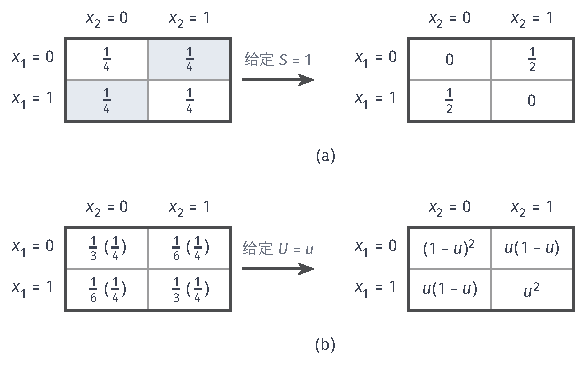
\includegraphics[width=98mm]{figures/07-probability/02-measure-theoretic-probability/tikz/cdis-ci-tables/figure.pdf}
  \caption{独立性随条件信息改变。(a)两枚独立公平硬币的联合概率表，浅蓝格子是事件$\{S=1\}$；给定$S=1$后只剩反对角线上的两格，$X_1$决定$X_2$。(b)随机硬币前两次抛掷的联合概率表，与各格边缘乘积（括号内）对照；给定$U=u$时表变为$u,1-u$的乘积表（右侧），条件独立而无条件不独立。}
  \label{fig:cdis-ci-tables}
\end{BookInlineFigure}

\paragraph{条件独立但不独立}
反方向用随机硬币。给定$U=u$时$X_1,X_2$独立，各以概率$u$为正面，所以$X_1\perp\!\!\!\perp X_2\mid U$。不给$U$时，由第~\ref{sec:cdis-chain}小节的公式，
\[
 \mathbb{P}(X_1=1,\ X_2=1)=\int_0^1u^{2}\,\mathrm{d}u=\frac13\neq\frac14=\mathbb{P}(X_1=1)\,\mathbb{P}(X_2=1).
\]
二者正相关，协方差为$\tfrac13-\tfrac14=\tfrac1{12}$，恰好是$\operatorname{Var}(U)$：两次抛掷共用同一个未知的正面概率，第一次的结果透露了$U$，于是影响对第二次的判断。

两个例子放在一起看。第一个例子中，$S$由$X_1,X_2$共同决定；把它加入条件，原本独立的两个量变得相关。第二个例子中，$U$同时影响$X_1,X_2$；把它从条件中去掉，原本条件独立的两个量变得相关。增加信息并不总是破坏独立：第二个例子中再给定$X_3$，即给定$(U,X_3)$，$X_1$与$X_2$仍然条件独立，因为给定$U$时三次抛掷相互独立。条件独立是$X$、$Z$与所给信息三者共同的性质，换了信息就要重新检查。

\paragraph{条件化与干预}
条件化回答的是“观测到$X_1=1$以后，对$X_2$的判断应当怎样修正”。随机硬币中，答案是把$\mathbb{P}(X_2=1)$从$\tfrac12$改成$\tfrac23$。另一个问题是：若有人不抛第一枚硬币，而是直接把它的记录写成正面，第二次抛掷的规律会怎样？这时硬币的正面概率$U$没有受到任何影响，第二次仍以$\tfrac12$的概率出现正面。

这两个问题的答案不同，而且第二个问题不能只靠联合分布回答。另一个模型是：第一次是公平硬币，第二次在第一次为正面时以$\tfrac23$、为反面时以$\tfrac13$出现正面。它与随机硬币的$(X_1,X_2)$有完全相同的联合分布，但在这个模型里改写第一次的记录，第二次正面的概率会变成$\tfrac23$。条件概率由联合规律决定；改变某个变量的产生方式以后会发生什么，还依赖产生数据的机制。研究这种操作的模型可参考\BookChapterRef{chap:causal-models-counterfactuals}{卷八第10章“因果模型与反事实”}。

\subsection{条件独立下的核复合}
\label{sec:cdis-composition}

设$X,Y,Z$都取值于标准Borel空间。已知给定$X$时$Y$的条件分布$K_{Y\mid X}$，以及给定$Y$时$Z$的条件分布$K_{Z\mid Y}$，能否得到给定$X$时$Z$的条件分布？一个自然的公式是先按$K_{Y\mid X}(x,\cdot)$抽出中间值$y$，再按$K_{Z\mid Y}(y,\cdot)$抽$z$，即对中间值积分。这个公式需要条件独立。

\begin{theorem}[核的复合]
\label{thm:cdis-composition}
设$X\perp\!\!\!\perp Z\mid Y$，$K_{Y\mid X}$与$K_{Z\mid Y}$分别是给定$X$时$Y$、给定$Y$时$Z$的正则条件分布。则
\begin{equation}
 L(x,C)=\int K_{Z\mid Y}(y,C)\,K_{Y\mid X}(x,\mathrm{d}y)
 \label{eq:cdis-composition}
\end{equation}
是给定$X$时$Z$的正则条件分布。
\end{theorem}

\begin{proof}
先说明$L$是概率核。固定$x$，$C\mapsto L(x,C)$非负、$L(x,\mathcal{Z})=1$；对两两不交的$C_n$，$K_{Z\mid Y}(y,\cup_nC_n)=\sum_nK_{Z\mid Y}(y,C_n)$，由单调收敛定理逐项积分，得到可数可加性。固定$C$，$y\mapsto K_{Z\mid Y}(y,C)$是有界可测函数，由定理~\ref{thm:cdis-kernel-product}第2条（被积函数只依赖$y$），$x\mapsto L(x,C)$可测。

再核对版本性质。固定$C$。依次用塔式法则（$\sigma(X)\subseteq\sigma(X,Y)$）、定理~\ref{thm:cdis-ci-markov}、正则条件分布$K_{Z\mid Y}$的定义，以及定理~\ref{thm:cdis-integral-representation}（对有界可测函数$y\mapsto K_{Z\mid Y}(y,C)$），得到
\[
 \begin{aligned}
 \mathbb{P}(Z\in C\mid X)
 &=\mathbb{E}\bigl[\mathbb{P}(Z\in C\mid X,Y)\bigm|X\bigr]
 =\mathbb{E}\bigl[\mathbb{P}(Z\in C\mid Y)\bigm|X\bigr]\\
 &=\mathbb{E}\bigl[K_{Z\mid Y}(Y,C)\bigm|X\bigr]\\
 &=\int K_{Z\mid Y}(y,C)\,K_{Y\mid X}(X,\mathrm{d}y)=L(X,C),
 \end{aligned}
\]
每个等号都几乎必然成立。
\end{proof}

式~\eqref{eq:cdis-composition}在有限状态时就是矩阵乘法。设$X$是房间的真实状态，$Y$是传感器读数，$Z$是传输到记录端的数值，都取$\{0,1\}$。读数只依据真实状态产生，记录只依据读数产生，转移矩阵为
\[
 \bm{W}_1=\begin{pmatrix}0.9&0.1\\0.2&0.8\end{pmatrix},\qquad
 \bm{W}_2=\begin{pmatrix}0.8&0.2\\0.3&0.7\end{pmatrix},
\]
第$i$行是给定上一级取值$i$时下一级的分布。

按第~\ref{sec:cdis-chain}小节的逐步构造，$Z$那一步的核只依赖$y$，所以$\mathbb{P}(Z\in C\mid X,Y)=\bm{W}_2$中第$Y$行在$C$上的和，它是$\sigma(Y)$可测的，于是也等于$\mathbb{P}(Z\in C\mid Y)$。由定理~\ref{thm:cdis-ci-markov}，$X\perp\!\!\!\perp Z\mid Y$。于是由式~\eqref{eq:cdis-composition}，给定$X$时$Z$的条件分布是
\[
 \bm{W}_1\bm{W}_2=\begin{pmatrix}0.9\cdot0.8+0.1\cdot0.3&0.9\cdot0.2+0.1\cdot0.7\\0.2\cdot0.8+0.8\cdot0.3&0.2\cdot0.2+0.8\cdot0.7\end{pmatrix}=\begin{pmatrix}0.75&0.25\\0.40&0.60\end{pmatrix}.
\]
真实状态为$0$时，记录正确的概率是$0.75$，由两条路径组成：读数正确且传输正确（$0.72$），读数错误且传输又出错（$0.03$）。图~\ref{fig:cdis-composition}(a)画出这些路径。

\begin{BookInlineFigure}
  \centering
  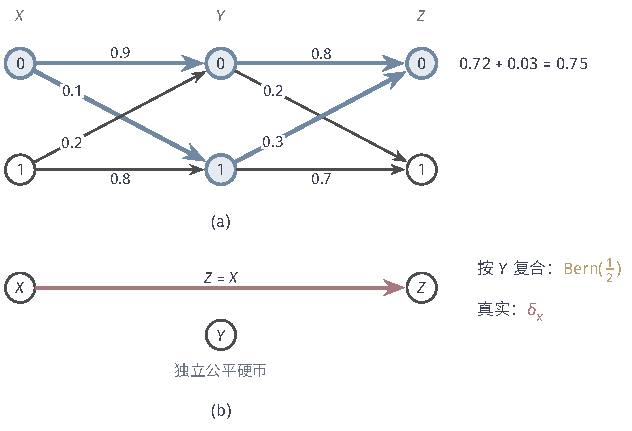
\includegraphics[width=107mm]{figures/07-probability/02-measure-theoretic-probability/tikz/cdis-composition/figure.pdf}
  \caption{核的复合。(a)$X\to Y\to Z$两级转移，边上是转移概率；从$X=0$到$Z=0$的两条路径（蓝）贡献$0.72$与$0.03$，合计$0.75$。(b)$Z=X$、$Y$为独立硬币时，按中间值$Y$复合得到$\operatorname{Bern}(\tfrac12)$（黄），而真实的条件分布是$\delta_x$（红）。}
  \label{fig:cdis-composition}
\end{BookInlineFigure}

\paragraph{条件独立不成立时}
复合公式不能直接用于任意三个随机变量。设$X,Y$是两枚独立的公平硬币，$Z=X$。给定$X$时$Y$仍是公平硬币；$Z=X$与$Y$独立，给定$Y$时$Z$也是公平硬币。按式~\eqref{eq:cdis-composition}复合，得到给定$X=x$时$Z\sim\operatorname{Bern}(\tfrac12)$；可是$Z=X$，真实的条件分布是$\delta_x$。错误在于$Z$与$X$的依赖并不经过$Y$：给定$Y$以后，$X$仍然完全决定$Z$，条件独立不成立。

复合公式对应的是一个两步构造：先有$X$，由$X$产生$Y$，再只由$Y$产生$Z$，依赖只通过中间变量传递。模型若按这种方式给出，条件独立由构造本身保证，复合可以放心使用；对已经给定的三个随机变量，必须先核对$X\perp\!\!\!\perp Z\mid Y$。


\section{本章小结}
\label{sec:cdis-summary}

本章开头问：没有概率表、没有密度，或者条件事件的概率为零时，“给定$Y=y$时$X$的分布”是什么。逐事件的条件概率，即指示函数的条件期望，总是存在，它是只依赖观测信息的随机变量，并且几乎必然满足概率的各条规则；但每条规则的例外集依赖所取的事件，不可数多个事件的版本随意挑选，可能在每个观测值处都拼不成分布。

概率核把这件事组织起来：固定观测值，它是一个概率测度；固定事件，它是观测值的可测函数。概率表中它就是行和为一的矩阵。正则条件分布是与联合规律相容的概率核，判别方法是按观测的分布把核积分回去，必须恢复每个矩形事件的联合概率。条件质量函数、条件密度以及$X=Y$时的单点分布$\delta_y$都通过这一判别。

存在性与唯一性都靠把要求压缩到可数个事件上。目标取实数值时，有理阈值上的分布函数值可数，例外集只并可数次，再用下确界补成分布函数；目标取值于标准Borel空间时，用Borel同构搬到实轴上。观测的取值空间不需要任何结构。两个正则条件分布在一个$P_Y$零测集之外相同，但联合规律不决定核在某个零概率观测值上的值。连续性等附加要求可以在零概率点上选出一个值，但满足要求的版本未必存在，选出的值还依赖用哪个观测量逼近，Borel--Kolmogorov悖论中带子与楔形给出$1$与$2x$两种答案。

表~\ref{tab:cdis-summary}对照了条件期望与条件分布。前者对任意可积随机变量存在，回答“给定信息后平均是多少”；后者要求目标空间有标准Borel结构，回答“给定信息后完整的规律是什么”，并通过积分给出前者的一个版本。

\begin{BookInlineTable}
  \centering
  \caption{条件期望与正则条件分布的对照}
  \label{tab:cdis-summary}
  \begin{tabular}{lll}
    \toprule
    & 条件期望$\mathbb{E}[g(X)\mid Y]$ & 正则条件分布$K(y,\cdot)$ \\
    \midrule
    对象 & 一个随机变量 & 每个$y$一个概率测度 \\
    定义 & 已知事件上积分相等 & 每个事件上取条件概率 \\
    存在 & $g(X)$可积即可 & 目标为标准Borel空间 \\
    唯一 & 几乎必然 & 在$P_Y$零测集之外 \\
    关系 & \multicolumn{2}{c}{$\mathbb{E}[g(X)\mid Y]=\int g(x)\,K(Y,\mathrm{d}x)$，$\mathbb{E}\lvert g(X)\rvert<\infty$} \\
    \bottomrule
  \end{tabular}
\end{BookInlineTable}

对核积分有两种方向。固定观测值、对目标积分，得到条件期望的积分表示，证明沿指示函数、简单函数、单调极限与正负分部进行；条件矩与条件方差就是条件分布的矩与方差。整体矩有限只保证条件矩几乎处处有限；反过来，每个观测值上条件矩有限也推不出整体矩有限。再按观测的分布积分，边缘与核唯一地确定联合规律，计算$f(X,Y)$的期望时可以把观测值代入、只对目标积分。对全部观测值积分得到全概率公式，从另一面看就是混合分布：随机硬币的正面次数是二项分布的均匀混合，t分布是高斯分布的尺度混合。

有限个标准Borel随机对象的联合规律总可以链式分解，每一步的核依赖此前的全部变量；反过来，起始分布和这样一列核唯一地确定一个联合规律，对应逐步的随机构造。在链式分解中省去条件变量，需要条件独立作为依据。

条件独立要求给定信息后对所有有界函数的乘积期望分解，等价于条件联合分布是条件边缘的乘积，也等价于已知条件后再知道$X$不改变$Z$的条件分布；条件协方差为零不够。独立与条件独立互不蕴含，增减条件信息都可能改变独立关系；条件化由联合规律决定，干预的效果还依赖产生数据的机制。给定中间变量条件独立时，核可以复合，有限状态下就是转移矩阵相乘；没有条件独立时复合会给出错误的答案。

这些工具在后面多处使用。给定观测后对未知量的分布作修正，是卷八统计推断的出发点，可参考\BookChapterRef{chap:parametric-statistical-inference}{卷八第1章“参数化统计推断”}。把链式分解与核复合沿时间无限地进行下去，就是随机过程中的转移结构，可参考\BookChapterRef{chap:discrete-time-stochastic-processes}{卷九第3章“离散时间随机过程”}。本卷在第~\ref{chap:sample-generation}章按核逐步产生样本，在第~\ref{chap:information-measures}章用条件分布定义条件熵与互信息。

